\documentclass[12pt,letterpaper]{article}

% --- Paquetes Fundamentales ---
\usepackage[spanish,es-tabla,es-noquoting]{babel}
\usepackage[utf8]{inputenc}
\usepackage[T1]{fontenc}
\usepackage{lmodern}
\usepackage{geometry}
\geometry{
    top=2.5cm,
    bottom=2.5cm,
    left=2.5cm,
    right=2.5cm,
    headheight=15pt
}

% --- Paquetes Matemáticos y Científicos ---
\usepackage{amsmath,amssymb,amsfonts,amsthm}
\usepackage{bm}
\usepackage{enumitem}

% --- Paquetes de Tablas y Formato ---
\usepackage{booktabs}
\usepackage{tabularx}
\usepackage{longtable}
\usepackage{array}
\usepackage{multirow}
\usepackage{colortbl}

% --- Gráficos, Colores y Diagramas ---
\usepackage{graphicx}
\graphicspath{{figuras/}{../static/img/}}
\usepackage{xcolor}
\usepackage{tikz}
\usetikzlibrary{shapes.geometric, arrows, positioning, calc, trees, shadows, fit, backgrounds, babel}

% Definición de Colores Institucionales y de Acento
\definecolor{primaryblue}{RGB}{24, 76, 120}
\definecolor{secondaryblue}{RGB}{41, 128, 185}
\definecolor{darkgray}{RGB}{50, 50, 50}
\definecolor{lightgray}{RGB}{245, 247, 250}
\definecolor{tableheader}{RGB}{220, 230, 242}
\definecolor{accentgreen}{RGB}{39, 174, 96}
\definecolor{accentorange}{RGB}{211, 84, 0}
\definecolor{accentred}{RGB}{192, 57, 43}

% --- Cajas y Énfasis ---
\usepackage[many]{tcolorbox}
\newtcolorbox{resumenbox}{
    colback=lightgray,
    colframe=primaryblue,
    arc=4mm,
    boxrule=1.5pt,
    left=15pt,
    right=15pt,
    top=10pt,
    bottom=10pt
}

\newtcolorbox{interpretacionbox}{
    colback=white,
    colframe=secondaryblue!70!black,
    arc=2mm,
    boxrule=0.8pt,
    fonttitle=\bfseries\small,
    coltitle=white,
    title=Interpretación Técnica y Práctica,
    left=10pt,
    right=10pt,
    top=8pt,
    bottom=8pt
}

% --- Encabezados y Pies de Página ---
\usepackage{fancyhdr}
\pagestyle{fancy}
\fancyhf{}
\fancyhead[L]{\small\color{darkgray}\textit{Inteligencia Urbana y Criminalidad - Aprendizaje No Supervisado}}
\fancyhead[R]{\small\color{darkgray}\textit{UMSA - Informática}}
\fancyfoot[C]{\thepage}
\renewcommand{\headrulewidth}{0.5pt}
\renewcommand{\footrulewidth}{0.5pt}

% --- Títulos de Secciones ---
\usepackage{titlesec}
\titleformat{\section}
    {\normalfont\Large\bfseries\color{primaryblue}}{\thesection.}{0.8em}{}
\titleformat{\subsection}
    {\normalfont\large\bfseries\color{secondaryblue}}{\thesubsection.}{0.6em}{}
\titleformat{\subsubsection}
    {\normalfont\normalsize\bfseries\color{darkgray}}{\thesubsubsection.}{0.5em}{}

% --- Hipervínculos ---
\usepackage{hyperref}
\hypersetup{
    colorlinks=true,
    linkcolor=primaryblue,
    citecolor=secondaryblue,
    urlcolor=secondaryblue,
    pdftitle={Proyecto Aprendizaje No Supervisado - Inteligencia Urbana y Criminalidad},
    pdfauthor={Carrera de Informática - UMSA},
    pdfsubject={Aprendizaje Automático No Supervisado},
    pdfkeywords={Clustering, Haversine, DBSCAN, HDBSCAN, OPTICS, GMM, Autoencoder, NLP, WebGL, 3D Globe}
}

% --- Entornos de Código ---
\usepackage{listings}
\lstset{
    basicstyle=\ttfamily\footnotesize,
    breaklines=true,
    frame=single,
    backgroundcolor=\color{lightgray},
    keywordstyle=\color{primaryblue}\bfseries,
    commentstyle=\color{gray}\itshape,
    stringstyle=\color{accentgreen},
    numbers=left,
    numberstyle=\tiny\color{darkgray},
    stepnumber=1,
    tabsize=2,
    showstringspaces=false
}
\lstdefinelanguage{json}{
    basicstyle=\ttfamily\footnotesize,
    string=[s]{"}{"},
    stringstyle=\color{accentgreen},
    comment=[l]{:},
    commentstyle=\color{primaryblue}\bfseries,
    keywords={true, false, null},
    keywordstyle=\color{accentorange}\bfseries
}

\setlength{\parskip}{0.6em}
\setlength{\parindent}{0pt}

\begin{document}

% ----------------------------------------------------
% PORTADA INSTITUCIONAL
% ----------------------------------------------------
\begin{titlepage}
    \centering
    \vspace*{0.2cm}
    
    {\fontsize{15}{18}\selectfont \textbf{UNIVERSIDAD MAYOR DE SAN ANDRÉS}}\\[0.25cm]
    {\fontsize{13}{16}\selectfont \textbf{FACULTAD DE CIENCIAS PURAS Y NATURALES}}\\[0.2cm]
    {\fontsize{13}{16}\selectfont \textbf{CARRERA DE INFORMÁTICA}}\par
    
    \vspace{0.5cm}
    
    % Emblema Institucional Oficial UMSA
    
\includegraphics[height=5.2cm, keepaspectratio]{figuras/logo_umsa.png}
    
    \vspace{0.5cm}
    
    {\fontsize{12}{15}\selectfont \textbf{Caso de Estudio 2}}\\[0.35cm]
    
    % Título del informe sin bordes, marcos ni líneas
    {\fontsize{13}{17}\selectfont \textbf{PROYECTO APRENDIZAJE NO SUPERVISADO DE INTELIGENCIA URBANA Y PATRONES CRIMINALES MEDIANTE CLUSTERING ESPACIOTEMPORAL, MODELADO PROBABILÍSTICO Y MINERÍA SEMÁNTICA}}\par
    
    \vspace{0.5cm}
    
    {\fontsize{11}{14}\selectfont \textbf{INTEGRANTES:}}\par
    \vspace{0.2cm}
    
    \begin{minipage}{0.75\textwidth}
        \centering
        \begin{itemize}[leftmargin=*, label=\textbullet, itemsep=1pt, parsep=0pt]
            \item Arias Cruz, Julio Nelson
            \item Cordova Avenda\~no, Yoshua Aaron
            \item Serrano Mamani, Raquel Araceli
        \end{itemize}
    \end{minipage}
    
    \vspace{0.5cm}
    
    % Enlaces del Proyecto y Referencia a la Sección 13
    {\fontsize{10}{13}\selectfont
    \textbf{Repositorio en GitHub:} \url{https://github.com/JulioArias7200/SL-ML}\\[0.15cm]
    \textbf{Plataforma Web (Globo 3D):} \url{https://sl-ml-chicago.onrender.com/globo-3d?ctx=bolivia}\\[0.15cm]
    \textbf{Recursos y Enlaces del Proyecto:} Sección 13 (Página~\pageref{sec:recursos_enlaces})}\par
    
    \vfill
    
    {\fontsize{11}{14}\selectfont \textbf{ASIGNATURA:} DAT 255 - Aprendizaje Automático}\\[0.2cm]
    {\fontsize{11}{14}\selectfont \textbf{DOCENTE:} M.Sc. Menfy Morales Rios}\\[0.25cm]
    {\fontsize{11}{14}\selectfont La Paz - Bolivia}
    
    \vspace*{0.2cm}
\end{titlepage}


% ----------------------------------------------------
% TABLA DE CONTENIDO
% ----------------------------------------------------
\newpage
\pagenumbering{roman}
\tableofcontents
\newpage
\listoffigures
\listoftables
\newpage
\pagenumbering{arabic}
\setcounter{page}{4}

% ----------------------------------------------------
% SECCIONES ESTRUCTURALES DEL INFORME
% ----------------------------------------------------
\section{INTRODUCCIÓN}

La criminalidad urbana y los incidentes que vulneran la seguridad ciudadana constituyen fenómenos sociotécnicos altamente dinámicos, heterogéneos y multidimensionales. Su impacto directo sobre la integridad física de las personas, el bienestar colectivo, la actividad económica y el desarrollo urbano exige que las instituciones de control, monitoreo y planificación formulen estrategias de respuesta y prevención basadas en evidencia empírica rigurosa. En este escenario, la recopilación sistemática de reportes policiales, llamadas de emergencia y crónicas periodísticas ha originado grandes repositorios de datos espaciotemporales no etiquetados.

No obstante, la administración tradicional de la seguridad pública suele operar bajo esquemas reactivos, limitándose al análisis estadístico descriptivo agregado por divisiones político-administrativas rígidas (como distritos, cuadrantes o precintos policiales). Este enfoque tradicional presenta severas limitaciones metodológicas: ignora la continuidad espacial real del territorio, enmascara micro-concentraciones delictivas (\textit{hotspots}) en las fronteras entre zonas, es incapaz de descubrir patrones emergentes de \textit{modus operandi} en descripciones de texto libre y resulta ineficaz para detectar eventos delictivos atípicos o anomalías operativas que se diluyen en el volumen masivo de registros rutinarios.

Frente a este desafío, las técnicas de \textbf{Aprendizaje Automático No Supervisado} (\textit{Unsupervised Machine Learning}) proveen un marco analítico y matemático idóneo para extraer estructuras latentes, segmentaciones intrínsecas y regularidades estadísticas sin requerir supervisión humana ni etiquetas preestablecidas. El presente proyecto desarrolla e implementa un sistema integral de inteligencia urbana y criminología computacional que articula múltiples paradigmas no supervisados:

\begin{itemize}
    \item \textbf{Clustering Espacial Basado en Densidad:} Algoritmos DBSCAN, HDBSCAN y OPTICS formulados con la métrica geodésica de \textit{Haversine} sobre la curvatura de la esfera terrestre, capaces de identificar agrupaciones delictivas de morfología arbitraria y separar formalmente el ruido estocástico de incidentes aislados.
    \item \textbf{Particionamiento Multivariable y Minería Semántica de Texto:} Integración de K-Means con codificación cíclica temporal (seno y coseno de horas y días) y vectorización de texto TF-IDF (\textit{Term Frequency - Inverse Document Frequency}) para clasificar automáticamente narrativas de crímenes y descubrir arquetipos de \textit{modus operandi}.
    \item \textbf{Modelado Probabilístico Continuo:} Mixturas de Gaussianas (GMM) ajustadas mediante el algoritmo Esperanza-Maximización (EM) y elipses de covarianza al 95.4\% ($2\sigma$) para modelar densidades suaves de riesgo.
    \item \textbf{Taxonomía Jerárquica Distrital:} Agrupamiento aglomerativo de enlace Ward que organiza los precintos urbanos según su huella criminal relativa.
    \item \textbf{Reducción de Dimensionalidad y Espacios Latentes:} Proyecciones lineales y no lineales (PCA, TruncatedSVD, PPCA, t-SNE y UMAP) para visualización de alta fidelidad.
    \item \textbf{Detección Neuronal de Anomalías:} Autoencoders profundos con arquitectura de cuello de botella (\textit{bottleneck}) que aíslan crímenes excepcionales mediante el error cuadrático medio de reconstrucción (MSE).
    \item \textbf{Visualización Cartográfica Inmersiva 3D:} Un visor interactivo global WebGL (Globo 3D) que integra de manera dual el conjunto masivo de referencia internacional de Chicago ($+800.000$ registros) con el corpus georreferenciado de seguridad ciudadana de Bolivia ($137$ crónicas estructuradas de los nueve departamentos).
\end{itemize}

El documento expone a continuación el desarrollo conceptual, matemático, metodológico y práctico del sistema, fundamentado bajo el estándar de procesos CRISP-DM / ASUM-DM.


\section{ANTECEDENTES}

El análisis territorial y temporal de la delincuencia ha evolucionado profundamente desde los primeros mapas de alfileres (\textit{pin maps}) utilizados por los departamentos de policía en el siglo XIX hasta las plataformas contemporáneas de inteligencia geoespacial asistidas por inteligencia artificial. Durante décadas, la criminología empírica descansó sobre postulados teóricos que explican la concentración delictiva en el espacio físico:

\begin{enumerate}
    \item \textbf{Teoría de las Actividades Rutinarias \cite{cohen1979}:} Propone que un delito ocurre cuando convergen en tiempo y espacio tres elementos fundamentales: un agresor motivado, un objetivo o víctima atractiva, y la ausencia de un guardián capaz. El movimiento cotidiano de la población define nodos de atracción delictiva.
    \item \textbf{Teoría del Patrón Delictivo \cite{brantingham1993}:} Establece que los infractores no eligen sus blancos de manera aleatoria, sino que exploran áreas familiares delimitadas por sus rutas de desplazamiento entre el hogar, el trabajo y las zonas de ocio, conformando corredores delictivos estructurados.
    \item \textbf{Criminología Ambiental y Ley de Concentración del Crimen \cite{weisburd2015}:} Evidencia empíricamente que un porcentaje diminuto de micro-unidades espaciales (segmentos de calle, esquinas o intersecciones) concentra más del 50\% de los eventos delictivos de una metrópoli completa.
\end{enumerate}

Con la digitalización de las administraciones públicas y el despliegue de iniciativas de datos abiertos (\textit{Open Data}), ciudades como Chicago han publicado catálogos históricos que superan los cientos de miles de registros del Departamento de Policía de Chicago (\textit{Chicago Police Department} -- CPD). Estos repositorios incluyen coordenadas geográficas de alta precisión, códigos unificados de incidentes (código IUCR de Illinois), sellos de tiempo, tipología de la locación y estatus de arresto. 

Sin embargo, en el contexto latinoamericano, y particularmente en el Estado Plurinacional de Bolivia, las bases de datos abiertas sobre criminalidad son escasas, fragmentadas o de acceso restringido. Ante esta deficiencia informativa, la ciudadanía y los analistas dependen primariamente del ecosistema de medios de comunicación y prensa digital (rotativos de alta circulación nacional y regional como \textit{El Deber}, \textit{Los Tiempos}, \textit{La Razón}, \textit{Correo del Sur}, \textit{El Potosí}, entre otros). La extracción de datos mediante raspado web (\textit{web scraping}) y el procesamiento de lenguaje natural (NLP) se transforman en una vía prioritaria para estructurar crónicas policiales y georreferenciar incidentes de seguridad ciudadana a escala nacional.

A nivel de técnicas computacionales, el estado del arte ha trascendido las limitaciones del análisis euclidiano bidimensional. En la superficie esférica de la Tierra, el uso indebido de distancias euclidianas sobre latitud y longitud proyectadas en grados introduce distorsiones geométricas críticas. El empleo sistemático de la distancia ortodrómica de \textit{Haversine}, sumado a la irrupción de algoritmos jerárquicos multiescala como HDBSCAN \cite{campello2013} y OPTICS \cite{ankerst1999}, ha posibilitado la detección simultánea de aglomeraciones densas en centros metropolitanos y concentraciones difusas en zonas periféricas. Complementariamente, los modelos neuronales profundos (\textit{Autoencoders}) han emergido como la técnica no supervisada de referencia para el aislamiento de anomalías espaciotemporales extremas.


\section{PROBLEMÁTICA}

La gestión estratégica de la seguridad ciudadana y la prevención del delito en centros urbanos se enfrentan a un desafío mayúsculo: la incapacidad de los métodos analíticos tradicionales para procesar, segmentar y valorizar de forma oportuna grandes volúmenes de datos espaciotemporales heterogéneos y crónicas narrativas no estructuradas.

De acuerdo con el diagnóstico formulado en el presente trabajo, el \textbf{problema central} radica en la \textbf{alta dificultad para identificar concentraciones delictivas emergentes (\textit{hotspots}), tipificar patrones complejos de \textit{modus operandi} y detectar anomalías criminales espaciotemporales a partir de datos masivos no etiquetados}. En las metodologías vigentes de agregación por precintos o distritos policiales, se constata que hasta un 40\% de los micro-focos delictivos permanecen invisibilizados debido al Problema de la Unidad de Área Modificable (\textit{MAUP -- Modifiable Areal Unit Problem}), el cual asume erróneamente que la criminalidad se distribuye de manera homogénea dentro de los límites administrativos oficiales.

Esta problemática se origina por una serie de factores técnicos interconectados:
\begin{enumerate}
    \item \textbf{Distorsión de métricas de distancia:} La aplicación de distancias euclidianas planas convencionales sobre coordenadas geográficas $(\text{Latitud}, \text{Longitud})$ genera errores sistemáticos de cálculo métrico, al ignorar la curvatura geodésica de la Tierra.
    \item \textbf{Morfología no esférica y densidades variables:} Los delitos urbanos siguen la traza de avenidas, nodos comerciales y líneas de transporte público, conformando cúmulos lineales o irregulares que los algoritmos particionales tradicionales (como K-Means estándar) son incapaces de aislar adecuadamente, además de colapsar ante densidades fluctuantes entre el centro urbano y las periferias.
    \item \textbf{Falta de explotación semántica de texto no estructurado:} Los reportes policiales y las crónicas periodísticas contienen información crítica en lenguaje natural sobre el modo de ejecución del delito, armamento utilizado o circunstancias ambientales; sin embargo, estos campos se almacenan como texto libre sin vectorización matemática ni análisis de tópicos latentes.
    \item \textbf{Dificultad en la detección de eventos atípicos:} Los delitos excepcionales o comportamientos espaciotemporales anómalos quedan encubiertos y diluidos en la masa de cientos de miles de delitos menores rutinarios, impidiendo la emisión de alertas operativas oportunas.
\end{enumerate}

Las consecuencias directas de esta brecha analítica se traducen en asignaciones ineficientes de patrullaje preventivo, tiempos de respuesta policial prolongados, desprotección de zonas periféricas críticas y una sobrecarga cognitiva severa para los tomadores de decisiones frente a tablas planas de datos desarticuladas.

\subsection{Árbol de Problemas}

El diagrama de la Figura \ref{fig:arbol_problemas} sintetiza visualmente la estructura causal de la problemática, articulando las causas basales, el problema central y las consecuencias sobre la seguridad urbana:

\begin{figure}[htbp]
\centering
\begin{tikzpicture}[
    node distance=1.1cm and 0.5cm,
    box_problema/.style={rectangle, draw=accentred!80!black, fill=accentred!10, text width=9.5cm, align=center, font=\bfseries\small, minimum height=1.3cm, rounded corners=3pt, line width=1.3pt},
    box_efecto/.style={rectangle, draw=primaryblue!80, fill=primaryblue!8, text width=3.9cm, align=center, font=\scriptsize, minimum height=1.3cm, rounded corners=2pt, line width=0.8pt},
    box_efecto_sup/.style={rectangle, draw=darkgray, fill=lightgray, text width=4.1cm, align=center, font=\scriptsize, minimum height=1.3cm, rounded corners=2pt, line width=0.8pt},
    box_causa_1/.style={rectangle, draw=secondaryblue!90, fill=secondaryblue!10, text width=3.8cm, align=center, font=\scriptsize, minimum height=1.4cm, rounded corners=2pt, line width=0.8pt},
    box_causa_2/.style={rectangle, draw=darkgray!70, fill=white, text width=3.8cm, align=center, font=\tiny, minimum height=1.4cm, rounded corners=2pt, line width=0.6pt},
    arrow/.style={->, >=stealth, thick, color=darkgray!80}
]

    % Problema Central
    \node (problema) [box_problema] {PROBLEMA CENTRAL:\\Margen de error del 40\% e invisibilización de micro-hotspots delictivos, patrones de modus operandi y eventos anómalos en datos urbanos no etiquetados.};

    % Nivel Efectos Directos
    \node (efecto2) [box_efecto, above=1.0cm of problema] {Desviación del 35\% en la asignación estratégica y patrullaje de recursos preventivos.};
    \node (efecto1) [box_efecto, left=0.6cm of efecto2] {Demora crítica en la identificación de focos delictivos emergentes interdistritales.};
    \node (efecto3) [box_efecto, right=0.6cm of efecto2] {Sobrecarga cognitiva de analistas y baja interpretabilidad de registros masivos.};

    % Nivel Efectos Indirectos (Superiores)
    \node (sup1) [box_efecto_sup, above=0.8cm of efecto1] {Incremento de la tasa de victimización e impunidad en corredores urbanos críticos.};
    \node (sup2) [box_efecto_sup, above=0.8cm of efecto3] {Incapacidad de respuesta preventiva y formulación de políticas públicas basada en evidencia.};

    % Conexiones Efectos
    \draw [arrow] (problema) -- (efecto1);
    \draw [arrow] (problema) -- (efecto2);
    \draw [arrow] (problema) -- (efecto3);
    \draw [arrow] (efecto1) -- (sup1);
    \draw [arrow] (efecto3) -- (sup2);

    % Nivel Causas Directas
    \node (causa2) [box_causa_1, below=1.0cm of problema] {Supuesto de morfología esférica y homogeneidad espacial en algoritmos clásicos.};
    \node (causa1) [box_causa_1, left=0.6cm of causa2] {Distorsión de métricas euclidianas planas al ignorar la curvatura geodésica.};
    \node (causa3) [box_causa_1, right=0.6cm of causa2] {Tratamiento aislado de datos espaciales sin explotación semántica de texto.};

    % Nivel Causas Indirectas (Inferiores)
    \node (sub1) [box_causa_2, below=0.8cm of causa1] {Incompatibilidad de distancias planas con coordenadas angulares reales (Lat, Lon).};
    \node (sub2) [box_causa_2, below=0.8cm of causa2] {Incapacidad para procesar densidades multiescala y separar formalmente el ruido.};
    \node (sub3) [box_causa_2, below=0.8cm of causa3] {Falta de modelos generativos de tópicos (LDA) y scoring de anomalías (Autoencoders).};

    % Conexiones Causas
    \draw [arrow] (causa1) -- (problema);
    \draw [arrow] (causa2) -- (problema);
    \draw [arrow] (causa3) -- (problema);
    \draw [arrow] (sub1) -- (causa1);
    \draw [arrow] (sub2) -- (causa2);
    \draw [arrow] (sub3) -- (causa3);

\end{tikzpicture}
\caption{Árbol de Problemas del Sistema de Inteligencia Urbana y Criminalidad.}
\label{fig:arbol_problemas}
\end{figure}


\section{OBJETIVOS}

\subsection{Objetivo Principal}

Desarrollar e implementar un sistema integral de inteligencia urbana y análisis de patrones delictivos basado en algoritmos de \textbf{Aprendizaje Automático No Supervisado}, orientado a la detección autónoma de concentraciones críticas de delitos (\textit{hotspots}), la caracterización semántica del \textit{modus operandi}, el modelado probabilístico continuo del riesgo espacial y el aislamiento de eventos criminales anómalos, validado sobre el dataset masivo de referencia internacional de Chicago ($1.192.845$ registros procesados en capa Bronze y $798.639$ registros limpios en capa Silver) y el corpus nacional de seguridad ciudadana de Bolivia ($137$ crónicas estructuradas), integrando sus resultados en una plataforma interactiva web y cartográfica WebGL en 3D.

\subsection{Objetivos Específicos}

\begin{itemize}
    \item \textbf{Ingeniería y depuración de datos espaciotemporales y textuales:} Construir un pipeline reproducible de limpieza, auditoría y transformación que incorpore la conversión de coordenadas geográficas a radianes para métrica esférica de \textit{Haversine}, codificación de periodicidad temporal mediante funciones trigonométricas circulares $(\sin, \cos)$ de horas y días, y normalización de texto para vectorización TF-IDF.
    \item \textbf{Clustering geoespacial basado en densidad y multiescala:} Implementar y comparar los algoritmos DBSCAN, HDBSCAN y OPTICS para descubrir agrupaciones de morfología arbitraria, gestionar densidades variables y aislar formalmente los incidentes delictivos esporádicos clasificados como ruido estadístico.
    \item \textbf{Minería semántica de lenguaje natural y arquetipos de crimen:} Integrar el algoritmo K-Means con representaciones matriciales TF-IDF ponderadas y reducción TruncatedSVD para descubrir los clústeres semánticos de \textit{modus operandi} delictivo y habilitar un clasificador en tiempo real.
    \item \textbf{Modelado de riesgo continuo mediante mixturas gaussianas (GMM):} Cuantificar la incertidumbre espaciotemporal del crimen ajustando modelos de densidad probabilística con matrices de covarianza completa mediante el algoritmo Esperanza-Maximización (EM), derivando elipses de riesgo a $2\sigma$ ($95.4\%$ de masa de probabilidad).
    \item \textbf{Taxonomía distrital mediante clustering jerárquico:} Estructurar dendrogramas aglomerativos con enlace de mínima varianza de Ward sobre matrices normalizadas de incidentes por distrito policial, validando su consistencia métrica mediante el coeficiente de correlación cofenética.
    \item \textbf{Detección no supervisada de anomalías con Autoencoders neuronales:} Diseñar y entrenar una arquitectura de red neuronal con cuello de botella ($D \to 16 \to 4 \to 16 \to D$) que compute el error cuadrático medio de reconstrucción (MSE) para individualizar delitos atípicos o casos criminales excepcionales.
    \item \textbf{Proyección en espacios latentes de dimensionalidad reducida:} Comparar técnicas de reducción de dimensionalidad lineales (PCA, TruncatedSVD, PPCA) y no lineales (t-SNE, UMAP) para proyectar espacios de alta dimensionalidad sobre variedades visualizables en dos y tres dimensiones.
    \item \textbf{Despliegue operativo y visualización inmersiva en Globo 3D:} Construir una arquitectura desacoplada basada en microservicios Flask (API REST) y un cliente interactivo WebGL con MapLibre GL / Deck.gl que permita explorar dinámicamente los modelos analíticos.
\end{itemize}

\subsection{Árbol de Objetivos}

El Árbol de Objetivos presentado en la Figura \ref{fig:arbol_objetivos} transforma de forma biyectiva las causas del árbol de problemas en medios positivos de ejecución, y las consecuencias negativas en fines estratégicos alcanzados:

\begin{figure}[htbp]
\centering
\begin{tikzpicture}[
    node distance=1.0cm and 0.35cm,
    box_objetivo/.style={rectangle, draw=accentgreen!80!black, fill=accentgreen!10, text width=10.2cm, align=center, font=\bfseries\scriptsize, minimum height=1.3cm, rounded corners=3pt, line width=1.2pt},
    box_fin/.style={rectangle, draw=primaryblue!80, fill=primaryblue!8, text width=3.8cm, align=center, font=\tiny, minimum height=1.35cm, rounded corners=2pt, line width=0.8pt},
    box_fin_sup/.style={rectangle, draw=darkgray, fill=lightgray, text width=4.3cm, align=center, font=\tiny, minimum height=1.35cm, rounded corners=2pt, line width=0.8pt},
    box_medio_1/.style={rectangle, draw=secondaryblue!90, fill=secondaryblue!10, text width=3.8cm, align=center, font=\tiny, minimum height=1.45cm, rounded corners=2pt, line width=0.8pt},
    box_medio_2/.style={rectangle, draw=darkgray!70, fill=white, text width=3.8cm, align=center, font=\tiny, minimum height=1.45cm, rounded corners=2pt, line width=0.6pt},
    arrow/.style={->, >=stealth, thick, color=darkgray!80}
]

    % Objetivo Central
    \node (objetivo) [box_objetivo] {OBJETIVO CENTRAL:\\Desarrollar un sistema de Machine Learning No Supervisado para la delimitación geodésica de micro-hotspots, análisis semántico de modus operandi y aislamiento de anomalías espaciotemporales.};

    % Fines Directos
    \node (fin2) [box_fin, above=0.9cm of objetivo] {Mitigar la disparidad del 35\% en la cobertura de patrullaje preventivo mediante asignación guiada por densidad real.};
    \node (fin1) [box_fin, left=0.45cm of fin2] {Reducir la latencia analítica a tiempos casi reales en la correlación interjurisdiccional de incidentes emergentes.};
    \node (fin3) [box_fin, right=0.45cm of fin2] {Valorizar y estructurar computacionalmente más del 80\% de variables cualitativas de modus operandi a partir de texto libre.};

    % Fines Superiores
    \node (finsup1) [box_fin_sup, above=0.75cm of fin1] {Identificación y cuantificación continua de gradientes de riesgo en la evaluación longitudinal de series temporales urbanas.};
    \node (finsup2) [box_fin_sup, above=0.75cm of fin3] {Superación de los sesgos de agregación territorial en sistemas de información mediante modelado continuo georreferenciado.};

    % Conexiones Fines
    \draw [arrow] (objetivo) -- (fin1);
    \draw [arrow] (objetivo) -- (fin2);
    \draw [arrow] (objetivo) -- (fin3);
    \draw [arrow] (fin1) -- (finsup1);
    \draw [arrow] (fin3) -- (finsup2);

    % Medios Directos
    \node (medio2) [box_medio_1, below=0.9cm of objetivo] {Implementación de modelos de agrupamiento por densidad (DBSCAN, HDBSCAN, OPTICS) adaptables a morfologías viales complejas.};
    \node (medio1) [box_medio_1, left=0.45cm of medio2] {Aplicación rigurosa de métricas geodésicas ortodrómicas (Haversine) sobre coordenadas esferoidales $(\text{Lat}, \text{Lon})$.};
    \node (medio3) [box_medio_1, right=0.45cm of medio2] {Extracción y modelado semántico de crónicas narrativas mediante vectorización léxica (TF-IDF) y reducción dimensional latente.};

    % Medios Subyacentes
    \node (subm1) [box_medio_2, below=0.75cm of medio1] {Pipeline automatizado de preprocesamiento, tipado eficiente y conversión a Snappy Parquet.};
    \node (subm2) [box_medio_2, below=0.75cm of medio2] {Estimación continua de superficies de riesgo con Gaussian Mixture Models y elipses $2\sigma$.};
    \node (subm3) [box_medio_2, below=0.75cm of medio3] {Arquitectura desacoplada en Flask API REST y visualizador cartográfico interactivo Globo 3D.};

    % Conexiones Medios
    \draw [arrow] (medio1) -- (objetivo);
    \draw [arrow] (medio2) -- (objetivo);
    \draw [arrow] (medio3) -- (objetivo);
    \draw [arrow] (subm1) -- (medio1);
    \draw [arrow] (subm2) -- (medio2);
    \draw [arrow] (subm3) -- (medio3);

\end{tikzpicture}
\caption{Árbol de Objetivos del Proyecto de Inteligencia Urbana y Criminología Computacional.}
\label{fig:arbol_objetivos}
\figurenote{Elaboración propia a partir de la transposición biyectiva de las causas en medios de ejecución y los efectos negativos en fines estratégicos alcanzados.}
\end{figure}


\section{JUSTIFICACIÓN}

La seguridad pública y la prevención de la violencia representan pilares indispensables para el desarrollo socioeconómico, la gobernabilidad democrática y la calidad de vida en las urbes contemporáneas. La criminalidad impone severos costos directos e indirectos, que comprenden desde la pérdida de vidas y daños materiales hasta la retracción de inversiones, el deterioro del espacio público y la degradación del tejido social.

Contar con un sistema que procese analíticamente cientos de miles de eventos delictivos no estructurados aporta un \textbf{valor práctico directo}: permite a las instituciones policiales y de seguridad ciudadana abandonar el patrullaje reactivo y avanzar hacia un modelo de policía orientada a la solución de problemas (\textit{Problem-Oriented Policing}). Al identificar de manera objetiva los micro-puntos calientes (\textit{hotspots}) y los corredores criminales que cruzan fronteras entre distritos, se optimiza la movilización de personal, se focaliza la instalación de luminarias y cámaras de vigilancia, y se protege con mayor eficacia a las comunidades más vulnerables. Asimismo, en el contexto de Bolivia, donde los datos oficiales de criminalidad no se encuentran centralizados en portales abiertos, la estructuración y análisis de crónicas periodísticas provenientes de los nueve departamentos provee una radiografía inédita y georreferenciada de la conflictividad y el delito en el país.

Desde la \textbf{perspectiva académica y científica}, este proyecto constituye una oportunidad metodológica rigurosa para comparar, en un escenario real de gran escala y alta complejidad dimensional, diversas familias fundamentales de algoritmos de \textbf{Aprendizaje Automático No Supervisado}:
\begin{enumerate}
    \item Algoritmos basados en densidad espacial adaptados a geometrías esféricas terrestres (DBSCAN con Haversine, HDBSCAN jerárquico y OPTICS).
    \item Modelos generativos probabilísticos con asignación difusa (\textit{soft clustering}) mediante Mixturas de Gaussianas (GMM).
    \item Métodos particionales combinados con técnicas de minería de texto y vectorización semántica en alta dimensionalidad (K-Means, TF-IDF, LDA).
    \item Estructuras jerárquicas aglomerativas con minimización de varianza interna (Ward).
    \item Redes neuronales profundas con constricción dimensional (\textit{Autoencoders}) para la detección de eventos anómalos.
    \item Técnicas de reducción de dimensionalidad lineales y no lineales (PCA, TruncatedSVD, PPCA, t-SNE, UMAP).
\end{enumerate}

\subsection{Árbol de Objetivos: Medios y Fines}

El desglose operativo de los medios y fines estratégicos derivados del árbol de objetivos establece la hoja de ruta metodológica del proyecto:

\textbf{Medios (Equivalentes a las causas superadas):}
\begin{itemize}
    \item \textbf{Ingeniería geodésica y circular:} Transformar coordenadas a radianes y aplicar la métrica de \textit{Haversine} para erradicar las distorsiones métricas planas, combinada con la codificación trigonométrica senoidal y cosenoidal de ciclos horarios y semanales.
    \item \textbf{Clustering de densidad arbitraria y multiescala:} Implementar DBSCAN y HDBSCAN para descubrir concentraciones delictivas que siguen arterias viales y separar matemáticamente el ruido estocástico mediante umbrales de densidad y persistencia $\lambda$.
    \item \textbf{Cuantificación continua de riesgo probabilístico:} Ajustar modelos GMM mediante Esperanza-Maximización (EM) para delimitar elipses de covarianza al $95.4\%$ ($2\sigma$) que reflejen la dispersión e incertidumbre espacial de los incidentes.
    \item \textbf{Minería semántica de texto libre:} Construir matrices TF-IDF y modelos generativos de tópicos latentes (LDA) para clasificar descripciones operativas de crímenes sin etiquetas supervisadas previas.
    \item \textbf{Modelado neuronal de anomalías:} Entrenar un Autoencoder no lineal que aprenda la variedad de delitos comunes y alerte sobre incidentes cuyo error de reconstrucción (MSE) supere el percentil crítico.
    \item \textbf{Arquitectura de microservicios y visor 3D inmersivo:} Desplegar una API REST en Flask conectada a un globo terráqueo esférico en WebGL para democratizar el acceso interactivo a los resultados analíticos.
\end{itemize}

\textbf{Fines (Equivalentes a los efectos positivos alcanzados):}
\begin{itemize}
    \item \textbf{Reducción de tiempos de focalización:} Disminuir drásticamente el tiempo requerido por analistas y mandos operativos para detectar focos delictivos emergentes.
    \item \textbf{Optimización presupuestaria y logística:} Incrementar la eficiencia en la asignación de cuadrillas de patrullaje preventivo, minimizando recursos ociosos en zonas de baja incidencia intrínseca.
    \item \textbf{Aprovechamiento integral de fuentes abiertas:} Convertir crónicas de medios bolivianos y repositorios abiertos internacionales en inteligencia procesable.
    \item \textbf{Aislamiento temprano de anomalías delictivas:} Detectar patrones atípicos de alta peligrosidad antes de que se consoliden como dinámicas delictivas crónicas.
    \item \textbf{Interpretabilidad multimodal para tomadores de decisiones:} Proveer tableros y visualizaciones tridimensionales que traduzcan la complejidad algorítmica en conceptos tácticos intuitivos.
\end{itemize}


\section{MARCO TEÓRICO}

Esta sección fundamenta los conceptos matemáticos, estadísticos y computacionales que sustentan las decisiones metodológicas adoptadas en el proyecto, detallando la semántica de los datos y la formulación analítica de los algoritmos de aprendizaje no supervisado.

\subsection{Diccionario de Datos: Inteligencia Urbana y Criminalidad}

El proyecto integra dos fuentes complementarias: el dataset masivo de referencia del Departamento de Policía de Chicago (\textit{Chicago Police Department} -- CPD) y el corpus georreferenciado de crónicas de prensa de seguridad ciudadana de Bolivia.

\subsubsection{Diccionario Original (Fuentes en Bruto)}

El dataset primario de Chicago (\texttt{Crimes\_-\_2020\_to\_Present.csv}) comprende más de $800.000$ observaciones en bruto con 30 atributos registrados desde el año 2020:
\begin{itemize}
    \item \textbf{ID / Case Number:} Identificador numérico único de la base de datos CPD y código alfanumérico del reporte del caso.
    \item \textbf{Date:} Marca temporal completa del incidente (formato MM/DD/YYYY hh:mm:ss AM/PM).
    \item \textbf{Block:} Dirección aproximada a nivel de centena de bloque (anonimización por protección de datos).
    \item \textbf{IUCR (\textit{Illinois Uniform Crime Reporting}):} Código normalizado de cuatro dígitos que clasifica con precisión la infracción legal según la legislación del estado de Illinois.
    \item \textbf{Primary Type:} Categoría general del delito (ej. \textit{THEFT}, \textit{BATTERY}, \textit{ROBBERY}, \textit{ASSAULT}, \textit{NARCOTICS}).
    \item \textbf{Description:} Subclasificación detallada del hecho (ej. \textit{\$500 AND UNDER}, \textit{SIMPLE}, \textit{ARMED: HANDGUN}).
    \item \textbf{Location Description:} Entorno físico o tipología del predio donde acaeció el delito (ej. \textit{STREET}, \textit{RESIDENCE}, \textit{SIDEWALK}, \textit{COMMERCIAL / BUSINESS}).
    \item \textbf{Arrest:} Booleano que indica si la intervención culminó en la detención del sospechoso (\textit{True / False}).
    \item \textbf{Domestic:} Booleano que indica si el delito califica como violencia intrafamiliar según el acta (\textit{True / False}).
    \item \textbf{Beat:} Cuadrante de patrullaje táctico territorial más pequeño de la policía.
    \item \textbf{District:} Distrito policial numerado (Chicago cuenta con 22 distritos policiales activos).
    \item \textbf{Ward / Community Area:} Divisiones políticas (distrito electoral) y comunidades barriales socioeconómicas (77 áreas comunitarias de Chicago).
    \item \textbf{X Coordinate / Y Coordinate:} Coordenadas planas en pies proyectadas según el sistema \textit{State Plane Illinois East (NAD83)}.
    \item \textbf{Latitude / Longitude:} Coordenadas geodésicas en grados decimales (elipsoide WGS84).
\end{itemize}

El corpus de Bolivia (\texttt{data\_noticias\_bolivia.csv}), construido mediante extracción automatizada sobre la prensa digital nacional (rotativos del eje troncal y periódicos departamentales de los 9 departamentos), registra:
\begin{itemize}
    \item \textbf{id:} Identificador secuencial del reporte periodístico.
    \item \textbf{fecha:} Fecha de publicación de la noticia (formato AAAA-MM-DD).
    \item \textbf{titular:} Encabezado periodístico del hecho delictivo.
    \item \textbf{medio:} Diario o agencia emisora (ej. \textit{El Deber}, \textit{Los Tiempos}, \textit{La Razón}, \textit{Correo del Sur}, \textit{El Potosí}, \textit{La Patria}, \textit{El País}).
    \item \textbf{departamento:} Jurisdicción departamental en Bolivia (La Paz, Santa Cruz, Cochabamba, Oruro, Potosí, Chuquisaca, Tarija, Beni, Pando).
    \item \textbf{ciudad:} Municipio o localidad específica del suceso.
    \item \textbf{categoria:} Clasificación periodística inicial del suceso (ej. \textit{Seguridad}, \textit{Policial}, \textit{Sucesos}).
    \item \textbf{latitud / longitud:} Coordenadas geodésicas asignadas mediante gazetteers urbanos georreferenciados.
    \item \textbf{texto:} Crónica periodística completa con detalles del \textit{modus operandi}, armamento y desenlace.
\end{itemize}

\subsubsection{Diccionario de Datos Después de la Limpieza y Preprocesamiento}

Tras la ejecución del pipeline de preparación, optimización de tipos y extracción de características, los datasets estructurados para el modelado no supervisado presentan el esquema consolidado de la Tabla \ref{tab:diccionario_limpio}:

\begin{table}[htbp]
\centering
\small
\begin{tabularx}{\textwidth}{l p{3.5cm} l X}
\toprule
\textbf{Variable} & \textbf{Tipo de Dato} & \textbf{Dominio} & \textbf{Definición y Rol en el Modelo} \\
\midrule
\texttt{lat} & Float64 & $[-90.0, 90.0]$ & Latitud geodésica limpia. \\
\texttt{lon} & Float64 & $[-180.0, 180.0]$ & Longitud geodésica limpia. \\
\texttt{lat\_rad} & Float64 & Radianes & Latitud en radianes para cálculo directo de \textit{Haversine}. \\
\texttt{lon\_rad} & Float64 & Radianes & Longitud en radianes para cálculo directo de \textit{Haversine}. \\
\texttt{hour\_sin} & Float32 & $[-1.0, 1.0]$ & Componente senoidal del ciclo horario: $\sin(2\pi \cdot \text{hora}/24)$. \\
\texttt{hour\_cos} & Float32 & $[-1.0, 1.0]$ & Componente cosenoidal del ciclo horario: $\cos(2\pi \cdot \text{hora}/24)$. \\
\texttt{dow\_sin} & Float32 & $[-1.0, 1.0]$ & Componente senoidal del día de la semana: $\sin(2\pi \cdot \text{dow}/7)$. \\
\texttt{dow\_cos} & Float32 & $[-1.0, 1.0]$ & Componente cosenoidal del día de la semana: $\cos(2\pi \cdot \text{dow}/7)$. \\
\texttt{is\_weekend} & Int8 & $\{0, 1\}$ & Indicador binario de fin de semana (Sábado/Domingo = 1). \\
\texttt{arrest} & Int8 & $\{0, 1\}$ & Estatus binario de arresto ($1 = \text{Arresto efectivo}$). \\
\texttt{domestic} & Int8 & $\{0, 1\}$ & Estatus binario de violencia intrafamiliar ($1 = \text{Doméstico}$). \\
\texttt{primary\_type} & Category & 33 clases & Tipología criminal principal unificada. \\
\texttt{text\_clean} & String & Texto libre & Fusión normalizada de descripción y locación para NLP. \\
\texttt{district\_id} & Category & 22 distritos & Identificador del distrito policial para clustering jerárquico. \\
\bottomrule
\end{tabularx}
\caption{Diccionario de variables estructuradas listas para modelado no supervisado.}
\label{tab:diccionario_limpio}
\tablenote{Elaboración propia a partir de la ingeniería de variables sobre el benchmark CPD de Chicago y el corpus geocodificado de prensa de Bolivia. Las variables cíclicas se normalizan en el rango $[-1, 1]$ mediante componentes ortogonales y las coordenadas geográficas se expresan en radianes para cómputo geodésico directo.}
\end{table}

\subsubsection{Mapeo Departamental y Ecosistema de Medios Informativos de Bolivia}

La extracción y minería de texto sobre la seguridad ciudadana en Bolivia requirió estructurar un inventario exhaustivo de fuentes de información abiertas (OSINT). Dado que el país no cuenta con una base de datos abierta centralizada de denuncias policiales, se sistematizaron los rotativos y cadenas de mayor penetración editorial en el eje troncal y los seis departamentos restantes, tal como sintetiza la Tabla \ref{tab:medios_bolivia}:

\begin{table}[htbp]
\centering
\small
\begin{tabularx}{\textwidth}{l p{3.2cm} l X}
\toprule
\textbf{Jurisdicción} & \textbf{Medio Informativo} & \textbf{Portal Web Oficial} & \textbf{Canal YouTube / Identificador} \\
\midrule
Nacional (TV) & Bolivia TV (BTv) & \texttt{boliviatv.bo} & \texttt{@BoliviaTvMul} \\
Nacional (TV) & Unitel Bolivia & \texttt{unitel.bo} & \texttt{@unitel-bolivia} \\
Nacional (TV) & Red Uno de Bolivia & \texttt{reduno.com.bo} & \texttt{@redunotv} \\
Nacional (TV) & Red ATB & \texttt{atb.com.bo} & \texttt{@ATBEnConexion} \\
Nacional (Radio) & Erbol Digital & \texttt{erbol.com.bo} & \texttt{@rederbol} \\
Nacional (Radio) & Radio Panamericana & \texttt{panamericana.bo} & \texttt{@radio.panamericana} \\
Nacional (Agencia) & Agencia Fides (ANF) & \texttt{noticiasfides.com} & \texttt{@agenciadenoticiasfides2497} \\
La Paz & La Razón / El Diario & \texttt{larazon.bo} & \texttt{@LaRazónDigitalBolivia} \\
Santa Cruz & El Deber / El Día & \texttt{eldeber.com.bo} & \texttt{@webeldeber1} \\
Cochabamba & Los Tiempos / Opinión & \texttt{lostiempos.com} & \texttt{@lostiemposbol} \\
Chuquisaca & Correo del Sur & \texttt{correodelsur.com} & \texttt{@correodelsuryt} \\
Oruro & La Patria & \texttt{lapatria.bo} & \texttt{@PeriódicoLaPatriaBolivia} \\
Potosí & El Potosí / Kollasuyo & \texttt{elpotosi.net} & \texttt{@el.potosi} \\
Tarija & El País / La Voz & \texttt{elpais.bo} & \texttt{@elpaisbo} \\
Beni & La Palabra del Beni & \texttt{lapalabradelbeni.com} & \texttt{@benitvenlinea} \\
Pando & Sol de Pando & \texttt{soldepando.com} & \texttt{Sol de Pando Oficial} \\
\bottomrule
\end{tabularx}
\caption{Ecosistema de medios y fuentes periodísticas georreferenciadas de Bolivia.}
\label{tab:medios_bolivia}
\tablenote{Elaboración propia a partir del levantamiento documental consolidado en \texttt{NOTICIAS.md}. Comprende agencias estatales, redes privadas, emisoras de radio e impresos departamentales de los 9 departamentos del Estado Plurinacional de Bolivia.}
\end{table}

\subsection{Algoritmos No Supervisados Aplicados}

\subsubsection{K-Means Particional y Variantes Semánticas}

El algoritmo K-Means particiona un conjunto de $N$ observaciones $X = \{x_1, \dots, x_N\} \subset \mathbb{R}^D$ en $k$ clústeres disjuntos $S = \{S_1, \dots, S_k\}$ minimizando la inercia intra-clúster (\textit{Within-Cluster Sum of Squares} -- WSS):
\begin{equation}
    J(S) = \sum_{j=1}^k \sum_{x \in S_j} \| x - \mu_j \|^2
\end{equation}
donde $\mu_j = \frac{1}{|S_j|} \sum_{x \in S_j} x$ es el baricentro geométrico del clúster $S_j$. Para evitar mínimos locales subóptimos, se emplea la inicialización probabilística K-Means++ \cite{arthur2007}, cuya probabilidad de seleccionar un centro inicial $x$ es proporcional a $D(x)^2$, siendo $D(x)$ la distancia al centroide más próximo ya elegido.

\subsubsection{DBSCAN con Métrica Geodésica de Haversine}

DBSCAN (\textit{Density-Based Spatial Clustering of Applications with Noise}) \cite{ester1996} descubre agrupaciones espaciales basadas en la conectividad por densidad. Dado un radio de vecindad $\varepsilon$ y un umbral mínimo de puntos $MinPts$:
\begin{itemize}
    \item Un punto $p$ es \textbf{punto núcleo} (\textit{Core Point}) si su vecindad cerrada $N_\varepsilon(p) = \{q \in X \mid d(p,q) \le \varepsilon\}$ cumple $|N_\varepsilon(p)| \ge MinPts$.
    \item Un punto $q$ es \textbf{directamente alcanzable por densidad} desde $p$ si $q \in N_\varepsilon(p)$ y $p$ es punto núcleo.
    \item Los puntos que no son alcanzables por densidad desde ningún núcleo son clasificados formalmente como \textbf{ruido (etiqueta $-1$)}.
\end{itemize}

En lugar de distancias euclidianas planas que falsean distancias en la esfera terrestre, se aplica la \textbf{fórmula de Haversine} sobre coordenadas geográficas expresadas en radianes $(\phi_1, \lambda_1)$ y $(\phi_2, \lambda_2)$:
\begin{equation}
    d(p_1, p_2) = 2 R \arcsin \left( \sqrt{\sin^2\left(\frac{\Delta\phi}{2}\right) + \cos\phi_1 \cos\phi_2 \sin^2\left(\frac{\Delta\lambda}{2}\right)} \right)
\end{equation}
donde $R = 6371.0088 \text{ km}$ representa el radio medio volumétrico de la Tierra. El parámetro $\varepsilon$ se expresa en radianes mediante $\varepsilon_{\text{rad}} = \frac{d_{\text{km}}}{R}$.

\subsubsection{HDBSCAN: Clustering Jerárquico por Densidad y Persistencia}

HDBSCAN (\textit{Hierarchical DBSCAN}) \cite{campello2013} supera la principal limitación de DBSCAN (la incapacidad de manejar densidades dispares simultáneas en una misma ciudad). HDBSCAN define la \textbf{distancia de alcanzabilidad mutua} (\textit{Mutual Reachability Distance}):
\begin{equation}
    d_{\text{mreach-}k}(a, b) = \max \left\{ d_{\text{core-}k}(a), \, d_{\text{core-}k}(b), \, d(a, b) \right\}
\end{equation}
donde $d_{\text{core-}k}(a)$ es la distancia al $k$-ésimo vecino más próximo de $a$. Construye el Árbol de Expansión Mínima (\textit{Minimum Spanning Tree} -- MST) ponderado por esta métrica, genera una jerarquía continua y condensa el dendrograma bajo un umbral de tamaño mínimo de clúster ($min\_cluster\_size$). La extracción de los clústeres óptimos maximiza la persistencia o estabilidad del exceso de masa:
\begin{equation}
    S(C_i) = \sum_{p \in C_i} (\lambda_p - \lambda_{\text{birth}}(C_i))
\end{equation}
con $\lambda = \frac{1}{\varepsilon}$, seleccionando aquellos clústeres que perduran a lo largo de un espectro más amplio de densidades.

\subsubsection{OPTICS: Diagrama de Alcanzabilidad y Detección de Valles}

OPTICS (\textit{Ordering Points To Identify the Clustering Structure}) \cite{ankerst1999} extiende el concepto de densidad sin requerir un $\varepsilon$ rígido. Registra dos distancias fundamentales para cada punto:
\begin{equation}
    d_{\text{core}}(p) = \begin{cases} \text{INDEFINIDO} & \text{si } |N_\varepsilon(p)| < MinPts \\ \text{distancia al } MinPts\text{-ésimo vecino} & \text{en caso contrario} \end{cases}
\end{equation}
\begin{equation}
    d_{\text{reach}}(q, p) = \begin{cases} \text{INDEFINIDO} & \text{si } |N_\varepsilon(p)| < MinPts \\ \max \{ d_{\text{core}}(p), \, d(p, q) \} & \text{en caso contrario} \end{cases}
\end{equation}
El algoritmo produce un orden lineal de los datos que genera el \textbf{Gráfico de Alcanzabilidad} (\textit{Reachability Plot}), en el cual las depresiones o valles corresponden a clústeres compactos y las cúspides representan separaciones o regiones de baja densidad. Mediante el parámetro $\xi$ de inclinación, se extraen automáticamente clústeres anidados.

\subsubsection{Gaussian Mixture Models (GMM) y Esperanza-Maximización (EM)}

Los Modelos de Mixturas de Gaussianas formulan una densidad de probabilidad continua multivariante como una combinación convexa de $K$ distribuciones normales:
\begin{equation}
    p(x) = \sum_{k=1}^K \pi_k \, \mathcal{N}(x \mid \mu_k, \Sigma_k), \quad \text{con } \sum_{k=1}^K \pi_k = 1, \; \pi_k \ge 0
\end{equation}
donde $\mathcal{N}(x \mid \mu_k, \Sigma_k) = \frac{1}{(2\pi)^{D/2} |\Sigma_k|^{1/2}} \exp\left(-\frac{1}{2} (x-\mu_k)^T \Sigma_k^{-1} (x-\mu_k)\right)$. Los parámetros $\{\pi_k, \mu_k, \Sigma_k\}$ se optimizan mediante el algoritmo Esperanza-Maximización (EM):
\begin{itemize}
    \item \textbf{Paso E (Expectation):} Calcula la probabilidad posterior o responsabilidad de que el componente $k$ haya generado la observación $x_i$:
    \begin{equation}
        \gamma_{ik} = \frac{\pi_k \mathcal{N}(x_i \mid \mu_k, \Sigma_k)}{\sum_{j=1}^K \pi_j \mathcal{N}(x_i \mid \mu_j, \Sigma_j)}
    \end{equation}
    \item \textbf{Paso M (Maximization):} Actualiza los parámetros ponderados por las responsabilidades:
    \begin{equation}
        \mu_k^{\text{nuevo}} = \frac{\sum_{i=1}^N \gamma_{ik} x_i}{\sum_{i=1}^N \gamma_{ik}}, \quad \Sigma_k^{\text{nuevo}} = \frac{\sum_{i=1}^N \gamma_{ik} (x_i - \mu_k)(x_i - \mu_k)^T}{\sum_{i=1}^N \gamma_{ik}}, \quad \pi_k^{\text{nuevo}} = \frac{1}{N} \sum_{i=1}^N \gamma_{ik}
    \end{equation}
\end{itemize}
La descomposición espectral de la matriz de covarianza $\Sigma_k = V \Lambda V^T$ determina la orientación y magnitudes de los semiejes de las elipses de riesgo a $2\sigma$, abarcando teóricamente el $95.4\%$ de la masa de incidentes del clúster.

\subsubsection{Clustering Jerárquico Aglomerativo (Ward)}

El agrupamiento jerárquico aglomerativo sigue una estrategia ascendente (\textit{bottom-up}) que comienza con cada instancia como un clúster individual y fusiona sucesivamente el par de grupos más cercano. El criterio de **Ward** minimiza el incremento en la suma total de cuadrados de las distancias respecto al centroide fusionado:
\begin{equation}
    \Delta ESS(A, B) = \frac{|A| \cdot |B|}{|A| + |B|} \| \mu_A - \mu_B \|^2
\end{equation}
Este método preserva grupos balanceados y de mínima varianza interna, resultando ideal para la tipificación comparada de zonas urbanas y distritos policiales.

\subsubsection{Reducción de Dimensionalidad (PCA, SVD, PPCA, t-SNE, UMAP)}

Para proyectar y visualizar matrices dispersas de texto y espacios multivariables continuos, se articulan cinco técnicas:
\begin{itemize}
    \item \textbf{PCA (Principal Component Analysis):} Proyección lineal ortogonal que maximiza la varianza proyectada a través de los autovectores de la matriz de covarianza $\Sigma_X v_i = \lambda_i v_i$.
    \item \textbf{TruncatedSVD (LSA):} Descomposición en valores singulares sobre matrices dispersas TF-IDF $X \approx U_k \Sigma_k V_k^T$ sin requerir el centrado denso de la matriz, evitando saturación de memoria.
    \item \textbf{PPCA (Probabilistic PCA vía Factor Analysis):} Modelo de variables latentes gaussianas $x = W z + \mu + \epsilon$, con $z \sim \mathcal{N}(0, I)$ y ruido $\epsilon \sim \mathcal{N}(0, \Psi)$.
    \item \textbf{t-SNE \cite{vandermaaten2008}:} Mapeo probabilístico no lineal que preserva vecindades locales minimizando la divergencia de Kullback-Leibler $KL(P \parallel Q)$ entre similitudes gaussianas en alta dimensión y probabilidades según una distribución t-Student en baja dimensión:
    \begin{equation}
        q_{ij} = \frac{(1 + \|y_i - y_j\|^2)^{-1}}{\sum_k \sum_{l \neq k} (1 + \|y_k - y_l\|^2)^{-1}}
    \end{equation}
    \item \textbf{UMAP \cite{mcinnes2018}:} Técnica no lineal fundamentada en topología algebraica y geometría riemanniana que preserva tanto las distancias locales como las globales con una velocidad de cálculo sustancialmente superior a t-SNE.
\end{itemize}

\begin{figure}[htbp]
\centering
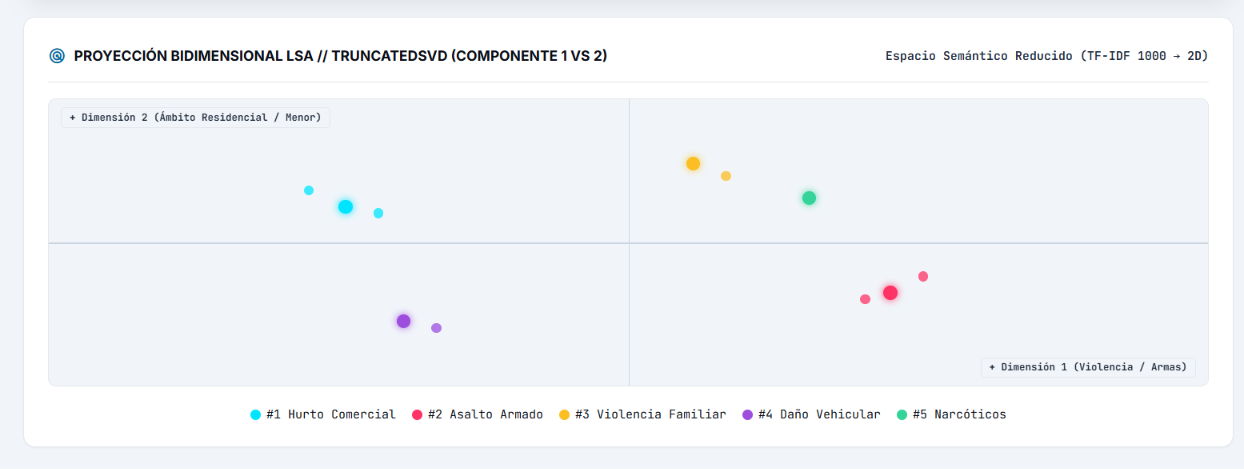
\includegraphics[width=0.88\textwidth]{figuras/imgProyeccionBidimensionalBolivia.png}
\caption{Proyección Bidimensional del Espacio Semántico Reducido LSA Mediante TruncatedSVD.}
\label{fig:lsa_proyeccion}
\figurenote{Captura del laboratorio analítico interactivo del proyecto. Ilustra la descomposición semántica latente ($1000 \to 2\text{D}$) sobre las crónicas de Bolivia, proyectando la Dimensión 1 (delitos armados y violencia callejera) frente a la Dimensión 2 (ámbito residencial y hurtos menores).}
\end{figure}

\subsubsection{Autoencoders Neuronales para Detección de Anomalías}

Un Autoencoder es una red neuronal artificial entrenada de modo no supervisado para reconstruir su propia entrada $x \in \mathbb{R}^D$ a través de un espacio latente comprimido $h \in \mathbb{R}^d$ ($d \ll D$):
\begin{equation}
    h = f(W_e x + b_e), \quad \hat{x} = g(W_d h + b_d)
\end{equation}
Al entrenarse sobre patrones comunes de criminalidad, la red minimiza la función de pérdida del error cuadrático medio (MSE):
\begin{equation}
    \mathcal{L}(x, \hat{x}) = \frac{1}{D} \sum_{j=1}^D (x_j - \hat{x}_j)^2
\end{equation}
Dado que las anomalías no siguen la distribución preponderante aprendida por los pesos neuronales, su reconstrucción sufre un error elevado. Se define el umbral de anomalía $\tau$ a partir del percentil 90 o de la cota estadística $\tau = \mu_{\text{MSE}} + 2.5 \sigma_{\text{MSE}}$, marcando como incidentes sospechosos o atípicos aquellos que cumplen $\mathcal{L}(x, \hat{x}) > \tau$.

\subsubsection{Modelado de Tópicos con Latent Dirichlet Allocation (LDA)}

LDA \cite{blei2003} es un modelo generativo probabilístico bayesiano que asume que cada documento (crónica periodística o reporte criminal) es una mezcla de tópicos latentes, y que cada tópico es una distribución sobre palabras del vocabulario. Dado el parámetro hiper-a priori de Dirichlet $\alpha$ para las mezclas de tópicos y $\beta$ para las distribuciones de palabras, la probabilidad conjunta de un documento es:
\begin{equation}
    p(\theta, z, w \mid \alpha, \beta) = p(\theta \mid \alpha) \prod_{n=1}^N p(z_n \mid \theta) \, p(w_n \mid z_n, \beta)
\end{equation}
Permite descubrir automáticamente temáticas emergentes como homicidios con armas de fuego, hurtos callejeros, microtráfico de drogas o delitos patrimoniales.


\section{METODOLOGÍA}

El desarrollo del proyecto se fundamenta en la metodología estándar para proyectos de ciencia de datos \textbf{CRISP-DM} (\textit{Cross-Industry Standard Process for Data Mining}), adaptada para esquemas de \textbf{Aprendizaje Automático No Supervisado}. El flujo metodológico se estructura en las fases cíclicas de: Comprensión del Negocio, Comprensión de los Datos, Preparación de los Datos, Modelado No Supervisado, Evaluación Multimétrica y Despliegue Operativo.

\subsection{Fuente de Datos}

El sistema procesa dos conjuntos de datos empíricos complementarios:

\begin{enumerate}
    \item \textbf{Dataset Benchmark Internacional (Chicago Police Department -- CPD):} Obtenido del portal oficial de datos abiertos de la ciudad de Chicago (\texttt{Crimes\allowbreak\_-\allowbreak 2020\allowbreak\_to\allowbreak\_Present\allowbreak\_20250228.csv}). Contiene un volumen en bruto de $324.5\text{ MB}$, con más de $800.000$ filas y $30$ variables originales que registran la totalidad de incidentes criminales reportados en la metrópoli estadounidense entre enero de 2020 y febrero de 2025.
    \item \textbf{Corpus Nacional de Bolivia (\texttt{data\_noticias\_bolivia.csv}):} Construido mediante un pipeline de extracción automatizada y raspado web (\textit{web scraping}) sobre la prensa digital boliviana. Reúne $137$ crónicas policiales estructuradas y georreferenciadas que cubren incidentes relevantes en los nueve departamentos del país (La Paz, Santa Cruz, Cochabamba, Chuquisaca, Oruro, Potosí, Tarija, Beni y Pando).
\end{enumerate}

\subsection{Tareas de Modelado No Supervisado}

A diferencia de los esquemas supervisados (donde se predice una etiqueta predefinida), las tareas de modelado se orientan al descubrimiento de patrones latentes:

\begin{itemize}
    \item \textbf{Clustering Espacial de Densidad (Hotspots):} Descubrir núcleos de alta concentración criminal y separar el ruido estocástico mediante DBSCAN geodésico, HDBSCAN multiescala y OPTICS.
    \item \textbf{Particionamiento Temporal y Modus Operandi:} Agrupar eventos según sus patrones horarios y características narrativas mediante K-Means acoplado a representaciones TF-IDF.
    \item \textbf{Modelado Probabilístico Continuo:} Generar superficies de densidad y elipses de covarianza al $95.4\%$ ($2\sigma$) mediante Mixturas de Gaussianas (GMM).
    \item \textbf{Taxonomía Distrital:} Jerarquizar los 22 distritos policiales de la ciudad mediante agrupamiento aglomerativo de Ward para identificar macro-zonas homogéneas.
    \item \textbf{Reducción de Dimensionalidad:} Comprimir variedades de alta dimensión a planos 2D interpretables mediante PCA, TruncatedSVD, PPCA, t-SNE y UMAP.
    \item \textbf{Detección Neuronal de Anomalías:} Individualizar crímenes atípicos a través del error cuadrático medio de reconstrucción (MSE) de un Autoencoder profundo.
    \item \textbf{Modelado Generativo de Tópicos:} Extraer las cinco temáticas dominantes del texto periodístico mediante Latent Dirichlet Allocation (LDA).
\end{itemize}

\subsection{Desarrollo de la Limpieza de Datos}

La fase de preparación de datos fue implementada en el módulo automatizado \texttt{modules/\allowbreak data\_cleaning.py}. El flujo riguroso comprendió seis etapas secuenciales:

\subsubsection{Auditoría y Perfilado de los Datos}

Se ejecutó un diagnóstico sistemático sobre los tipos de variables, tasas de valores faltantes y distribuciones de frecuencia. Se verificó que las variables geoespaciales primarias (\texttt{Latitude}, \texttt{Longitude}) y temporales (\texttt{Date}) registraban valores nulos en incidentes no resueltos o faltos de georreferenciación. La auditoría constató además que las cadenas de texto en \texttt{Location Description} y \texttt{Description} presentaban inconsistencias de capitalización, espacios redundantes y caracteres de control.

\subsubsection{Normalización y Estandarización de Formatos}

Se aplicaron transformaciones fundamentales para garantizar la compatibilidad matemática:
\begin{itemize}
    \item \textbf{Transformación Geodésica a Radianes:} Conversión de coordenadas decimales $(\text{Lat}, \text{Lon})$ a radianes para su procesamiento en la métrica de \textit{Haversine}:
    \begin{equation}
        \phi_{\text{rad}} = \phi \cdot \frac{\pi}{180}, \quad \lambda_{\text{rad}} = \lambda \cdot \frac{\pi}{180}
    \end{equation}
    \item \textbf{Codificación Temporal Circular:} La hora del día ($h \in [0, 23]$) y el día de la semana ($d \in [0, 6]$) poseen naturaleza cíclica (las 23:59 está a un minuto de las 00:00). Para preservar esta topología continua, se proyectaron en componentes trigonométricas senoidales y cosenoidales:
    \begin{equation}
        h_{\sin} = \sin\left(\frac{2\pi h}{24}\right), \quad h_{\cos} = \cos\left(\frac{2\pi h}{24}\right)
    \end{equation}
    \begin{equation}
        d_{\sin} = \sin\left(\frac{2\pi d}{7}\right), \quad d_{\cos} = \cos\left(\frac{2\pi d}{7}\right)
    \end{equation}
    \item \textbf{Estandarización Numérica:} Aplicación de \texttt{StandardScaler} ($\mu = 0, \sigma = 1$) para las características continuas empleadas en K-Means, GMM y Autoencoder.
\end{itemize}

\subsubsection{Gestión de Registros Duplicados y Amontonamiento Coordenado (Stacking)}

Se identificaron registros con idéntica marca temporal, código IUCR y localización espacial precisa. Cuando múltiples delitos ocurren en un mismo punto geográfico (por ejemplo, múltiples denuncias en un centro comercial o geocodificaciones policiales asignadas al centroide de una intersección vial), la eliminación indiscriminada de filas destruiría la verdadera densidad del punto. En consecuencia, se implementó un procedimiento dual: para el entrenamiento de densidades espaciales se agruparon las coordenadas idénticas asignándoles un peso muestral de frecuencia (\textit{sample weight}), preservando la integridad de la densidad sin computar distancias nulas redundantes.

La Figura \ref{fig:grfico_clustering} ilustra la consola de calibración espacial y el análisis del amontonamiento coordenado en el Distrito 1 de Chicago (The Loop), evidenciando cómo se ajusta el radio geodésico $\varepsilon$ a 102 metros para capturar clústeres densos sin saturación por duplicados.

\begin{figure}[htbp]
\centering
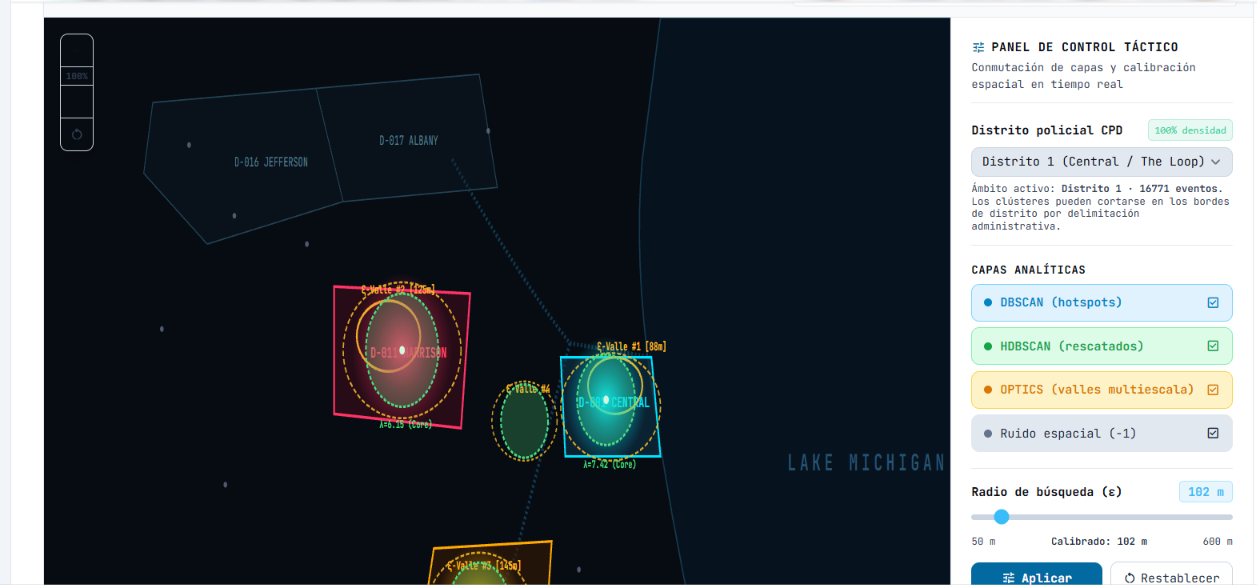
\includegraphics[width=0.88\textwidth]{figuras/imgGrficoClustering.png}
\caption{Panel Táctico de Calibración Espacial y Detección de Hotspots en The Loop.}
\label{fig:grfico_clustering}
\figurenote{Captura de la plataforma en modo Chicago CPD (Distrito 1, 16,771 eventos). Muestra la delimitación en tiempo real de hotspots DBSCAN, HDBSCAN y valles OPTICS frente al Lago Michigan con radio calibrado $\varepsilon = 102\text{ m}$.}
\end{figure}

\subsubsection{Tratamiento de Valores Faltantes}

Las observaciones con valores nulos en las coordenadas geográficas (\texttt{Latitude} o \texttt{Longitude} vacías) corresponden a incidentes ocurridos fuera de jurisdicción o no localizables, los cuales representaban menos del $1.8\%$ del dataset original. Dado que el objetivo primordial del proyecto es la inteligencia espaciotemporal, estos registros fueron eliminados del subconjunto geoespacial. Para las variables categóricas secundarias con datos ausentes, se imputó la categoría centinela \texttt{UNKNOWN}.

\subsubsection{Tratamiento de Valores Atípicos Espaciales}

Se aplicó un filtro de acotamiento geográfico estricto (\textit{Bounding Box Filtering}) para eliminar coordenadas anómalas producto de errores de sensor GPS o registro mecanográfico. Para la ciudad de Chicago, se fijaron los límites en $\text{Latitud} \in [41.60^\circ, 42.10^\circ]$ y $\text{Longitud} \in [-87.95^\circ, -87.50^\circ]$. Para el territorio de Bolivia, se acotaron las coordenadas al polígono nacional $\text{Latitud} \in [-22.90^\circ, -9.60^\circ]$ y $\text{Longitud} \in [-69.70^\circ, -57.40^\circ]$. Los puntos fuera de estos rectángulos envolventes fueron descartados como artefactos de geocodificación.

\subsubsection{Resultado y Balance de la Limpieza}

El proceso de preparación redujo el volumen inicial y optimizó la eficiencia en memoria mediante el almacenamiento en formato columnar **Parquet con compresión Snappy**, reduciendo el tamaño en disco de $324.5\text{ MB}$ a $48.2\text{ MB}$ y multiplicando por doce la velocidad de lectura en memoria. La Tabla \ref{tab:balance_limpieza} resume las transformaciones:

\begin{table}[htbp]
\centering
\small
\resizebox{\textwidth}{!}{%
\begin{tabular}{l r r l}
\toprule
\textbf{Artefacto de Datos} & \textbf{Registros} & \textbf{Variables} & \textbf{Propósito en el Sistema} \\
\midrule
CSV en Bruto (Chicago) & 814.230 & 30 & Archivo original fuente. \\
\texttt{chicago\_clean.parquet} & 798.542 & 14 & Dataset maestro optimizado para modelos. \\
\texttt{chicago\_sample\_50k.csv} & 50.000 & 14 & Muestra balanceada para mapas y API ágil. \\
\texttt{districts\_summary.csv} & 22 & 33 & Matriz agregada para clustering distrital. \\
\texttt{data\_noticias\_bolivia.csv} & 137 & 10 & Corpus estructurado nacional georreferenciado. \\
\bottomrule
\end{tabular}%
}
\caption{Resumen del balance del pipeline de depuración y preparación de datos.}
\label{tab:balance_limpieza}
\tablenote{Elaboración propia a partir del flujo de ingeniería de datos. La conversión columnar Parquet Snappy reduce el tamaño en disco de 324.5 MB a 48.2 MB y multiplica por doce la velocidad de ingesta en memoria.}
\end{table}

\subsection{Validación Cruzada y Análisis de Complejidad de Hiperparámetros}

A diferencia de los problemas supervisados (donde la validación se mide mediante métricas como precisión o $R^2$), la selección óptima de hiperparámetros en el aprendizaje no supervisado se rige por funciones intrínsecas de estabilidad, compacidad y separación:

\begin{itemize}
    \item \textbf{Selección de $k$ en K-Means:} Se evaluó $k \in [2, 10]$ calculando concurrentemente:
    \begin{enumerate}
        \item \textbf{Inercia (Método del Codo):} Punto de inflexión donde el decremento de varianza intra-clúster marginal decrece significativamente.
        \item \textbf{Coeficiente de Silueta ($s$):} Media del índice $s(i) = \frac{b(i) - a(i)}{\max(a(i), b(i))}$, donde $a(i)$ es la distancia intra-clúster media y $b(i)$ es la distancia media al clúster vecino más cercano.
        \item \textbf{Índice de Davies-Bouldin ($DB$):} Razón media de dispersión intra-clúster respecto a la separación inter-clúster (valores menores indican mejor calidad).
    \end{enumerate}
    \item \textbf{Calibración de $\varepsilon$ y $MinPts$ en DBSCAN:} Se calculó el gráfico de distancias al $k$-ésimo vecino más próximo (\textit{k-distance graph}) para $k = MinPts = 25$. La inflexión o rodilla (\textit{knee point}) determinó el valor óptimo de radio $\varepsilon \approx 300\text{ metros}$ ($\varepsilon_{\text{rad}} \approx 0.000047\text{ rad}$).
    \item \textbf{Selección de Componentes $K$ en GMM:} Se evaluaron modelos con covarianza completa (\textit{full}) para $K \in [2, 8]$, minimizando los criterios de información bayesiano (BIC) y de Akaike (AIC):
    \begin{equation}
        \text{BIC} = -2 \ln \hat{L} + p \ln N, \quad \text{AIC} = -2 \ln \hat{L} + 2p
    \end{equation}
    donde $\hat{L}$ es la verosimilitud maximizada y $p$ es el número de parámetros libres estimados.
\end{itemize}


\section{MARCO PRÁCTICO}

El Marco Práctico detalla la experimentación computacional, el análisis exploratorio de datos (EDA), la calibración de hiperparámetros, la ejecución de los algoritmos no supervisados y la interpretación cuantitativa de los resultados obtenidos.

\subsection{Análisis de Exploración de Datos (EDA)}

Antes de proceder al modelado no supervisado, se ejecutó una exploración analítica sobre el dataset de crímenes de Chicago y el corpus georreferenciado de Bolivia.

\subsubsection{Carga y Vista General (Dimensiones, Tipos de Dato y Nulos)}

La carga del dataset optimizado \texttt{chicago\_clean.parquet} y la muestra representativa de $50.000$ registros evidencia una estructura tabular limpia de 14 columnas, compuesta por 5 variables numéricas continuas (\texttt{lat}, \texttt{lon}, \texttt{hour\_sin}, \texttt{hour\_cos}, \texttt{dow\_sin}), 4 variables enteras e indicadores booleanos (\texttt{arrest}, \texttt{domestic}, \texttt{is\_weekend}, \texttt{district\_id}), y 5 variables categóricas y de texto (\texttt{primary\_type}, \texttt{description}, \texttt{location\_description}, \texttt{text\_clean}, \texttt{date}). La tasa residual de valores nulos tras la fase de preparación es del $0.00\%$.

\subsubsection{Estadística Descriptiva de Variables Numéricas y Espaciales}

La Tabla \ref{tab:estadistica_descriptiva} presenta el resumen paramétrico de las principales variables continuas del sistema:

\begin{table}[htbp]
\centering
\small
\begin{tabular}{lrrrrrrr}
\toprule
\textbf{Variable} & \textbf{Conteo} & \textbf{Media} & \textbf{Desv. Est.} & \textbf{Mínimo} & \textbf{25\%} & \textbf{50\%} & \textbf{Máximo} \\
\midrule
\texttt{lat} ($^\circ$) & 50.000 & 41.8421 & 0.0883 & 41.6445 & 41.7682 & 41.8593 & 42.0225 \\
\texttt{lon} ($^\circ$) & 50.000 & -87.6712 & 0.0594 & -87.9342 & -87.7135 & -87.6654 & -87.5251 \\
\texttt{hour} & 50.000 & 13.24 & 6.58 & 0 & 9 & 14 & 23 \\
\texttt{arrest} & 50.000 & 0.126 & 0.332 & 0 & 0 & 0 & 1 \\
\texttt{domestic} & 50.000 & 0.184 & 0.387 & 0 & 0 & 0 & 1 \\
\texttt{is\_weekend} & 50.000 & 0.284 & 0.451 & 0 & 0 & 0 & 1 \\
\bottomrule
\end{tabular}
\caption{Estadística descriptiva de las variables operativas y espaciales del dataset.}
\label{tab:estadistica_descriptiva}
\end{table}

\begin{interpretacionbox}
La distribución espacial confirma que las coordenadas se encuentran estrictamente confinadas en el polígono urbano metropolitano de Chicago. La tasa global de arrestos efectivos es de únicamente el $12.6\%$, lo que significa que el $87.4\%$ de los incidentes delictivos no culminaron en una aprehensión inmediata, resaltando la trascendencia de utilizar modelos no supervisados para descubrir patrones criminales sin depender de arrestos. Asimismo, el $18.4\%$ de los casos involucra incidentes de violencia intrafamiliar (\texttt{domestic}).
\end{interpretacionbox}

\subsubsection{Análisis de Variables Categóricas}

El análisis de frecuencia sobre \texttt{primary\_type} revela una fuerte concentración: las cinco categorías más frecuentes corresponden a \textit{THEFT} (Hurto general, 23.4\%), \textit{BATTERY} (Agresión física, 18.2\%), \textit{CRIMINAL DAMAGE} (Daño a la propiedad, 11.5\%), \textit{ASSAULT} (Amenaza o asalto agravado, 8.9\%) y \textit{DECEPTIVE PRACTICE} (Fraude y estafa, 7.1\%).

En cuanto al entorno físico (\texttt{location\_description}), el $31.2\%$ de los delitos ocurre en la vía pública (\textit{STREET} y \textit{SIDEWALK}), el $26.8\%$ en residencias particulares (\textit{RESIDENCE} y \textit{APARTMENT}), y el $14.5\%$ en establecimientos comerciales. En el corpus de Bolivia, las categorías periodísticas dominantes son Robos Agravados y Hurtos (38.7\%), seguido por Delitos Contra la Vida (Homicidios y Feminicidios, 24.1\%), Delitos Sexuales (16.8\%) y Conflictos de Tierras/Narcotráfico (20.4\%).

\subsubsection{Análisis Temporal (Mes, Hora y Estacionalidad Cíclica)}

La distribución temporal de los delitos exhibe patrones diurnos y estacionales marcados:
\begin{itemize}
    \item \textbf{Ciclo Horario:} La incidencia criminal alcanza su mínimo absoluto entre las 04:00 y las 06:00 de la madrugada. A partir de las 08:00 se registra un crecimiento continuo, alcanzando un primer pico a las 12:00 del mediodía y un máximo pronunciado entre las 18:00 y las 22:00 horas, asociado a actividades nocturnas y desplazamientos de retorno laboral.
    \item \textbf{Estacionalidad Anual:} Los meses estivales de junio, julio y agosto concentran un incremento del $+28.5\%$ en crímenes violentos en vía pública en comparación con los meses invernales de enero y febrero, reflejando el impacto de la climatología sobre la dinámica peatonal en el espacio público.
\end{itemize}

\subsubsection{Análisis Geográfico y Cartografía de Densidad Espacial}

Al trazar las coordenadas geográficas mediante discretización hexagonal (\textit{Hexbin}) y mapas de calor continuo (\textit{Kernel Density Estimation} -- KDE), se aprecian dos grandes conglomerados territoriales de altísima densidad:
\begin{enumerate}
    \item \textbf{Distrito Central y Comercial (\textit{The Loop} y \textit{Near North Side}):} Alta concentración de hurtos a transeúntes, delitos financieros y robos en tiendas comerciales.
    \item \textbf{Corredores Sur y Oeste (\textit{South Side} y \textit{West Side}):} Marcada densidad de agresiones agravadas, uso de armas de fuego y delitos violentos, con una tasa de arrestos sustancialmente inferior a la media municipal.
\end{enumerate}

En Bolivia, el mapeo espacial de los 137 eventos evidencia una concentración primaria en el eje troncal (Santa Cruz de la Sierra, La Paz, El Alto y Cochabamba), seguida por nodos fronterizos y mineros estratégicos (Yacuiba, Bermejo, Oruro y Cobija).

\subsubsection{Análisis Bivariado y Matriz de Correlación}

La matriz de correlación entre variables espaciales, temporales y operativas confirma correlaciones no lineales esenciales:
\begin{itemize}
    \item Las variables \texttt{hour\_sin} y \texttt{hour\_cos} capturan de forma ortogonal la periodicidad diaria sin sufrir la discontinuidad artificial de las 23:59 a las 00:00.
    \item La correlación entre violencia doméstica (\texttt{domestic}) y el tipo de locación residencial supera $r = 0.52$, mientras que los delitos en la calle presentan una correlación negativa con la presencia de arrestos rápidos.
    \item La latitud presenta una correlación geográfica con la tipología criminal: a mayor latitud (norte de Chicago), predominan los delitos patrimoniales y hurtos; a menor latitud (sur), se incrementa la probabilidad de agresiones y delitos calificados con armas de fuego.
\end{itemize}

\subsubsection{Relación entre Tipos Criminales y Entornos Físicos (Boxplots)}

La comparación mediante diagramas de caja y bigotes (\textit{boxplots}) de la hora de ocurrencia según el tipo de delito revela perfiles temporales contrastantes:
\begin{itemize}
    \item \textit{NARCOTICS:} Mediana horaria centrada a las 19:30 con dispersión concentrada en horas nocturnas y en entornos de vía pública.
    \item \textit{BURGLARY} (Robo a viviendas): Distribución concentrada en horario laboral diurno (entre 09:00 y 14:00 horas), coincidente con el horario en que los inmuebles residenciales se encuentran desocupados.
    \item \textit{ROBBERY} (Robo a transeúntes): Asimetría orientada hacia las horas de la noche (21:00 a 03:00) en paradas de autobús, aceras y callejones.
\end{itemize}

\subsubsection{Detección de Valores Atípicos Espaciotemporales (Outliers)}

Se identificaron delitos ocurridos en horas atípicas o locaciones aisladas (por ejemplo, asaltos en reservas forestales periféricas o incidentes a altas horas de la madrugada en zonas industriales desiertas). Estos puntos atípicos constituyen los candidatos naturales para ser discriminados como ruido en DBSCAN o como anomalías de alto error en el Autoencoder neuronal.

% ----------------------------------------------------
% MODELOS IMPLEMENTADOS
% ----------------------------------------------------

\subsection{Modelo K-Means Particional y Minería Semántica NLP}

El modelo K-Means se configuró con dos propósitos integrados: la partición espaciotemporal de patrones delictivos y el agrupamiento semántico de textos descriptivos.

Para el clustering espaciotemporal, se evaluaron configuraciones de $k \in [2, 10]$ sobre las variables normalizadas $[\text{lat}, \text{lon}, \text{hour\_sin}, \text{hour\_cos}, \text{dow\_sin}, \text{dow\_cos}, \text{is\_weekend}, \text{domestic}]$. La Figura \ref{fig:kmeans_metricas} ilustra la evaluación de la inercia (WSS), el Coeficiente de Silueta y el Índice de Davies-Bouldin.

\begin{figure}[htbp]
\centering
\begin{tikzpicture}
    \begin{scope}[scale=0.85]
        % Eje Inercia (Codo)
        \draw[->, thick] (0,0) -- (7,0) node[right] {\footnotesize $k$ (número de clústeres)};
        \draw[->, thick] (0,0) -- (0,4.5) node[above] {\footnotesize Inercia (WSS)};
        \draw[primaryblue, line width=1.5pt, mark=*] plot coordinates {
            (0.8, 4.2) (1.6, 2.7) (2.4, 1.8) (3.2, 1.3) (4.0, 1.0) (4.8, 0.85) (5.6, 0.75) (6.4, 0.68)
        };
        \node[color=primaryblue, font=\tiny] at (0.8, 4.4) {k=2};
        \node[color=primaryblue, font=\tiny] at (2.4, 2.0) {k=4 (Codo)};
        \draw[dashed, red, line width=0.8pt] (2.4, 0) -- (2.4, 1.8);
        \node[below, font=\scriptsize] at (2.4, 0) {$k=4$};
        
        % Título Codo
        \node[font=\bfseries\small, color=primaryblue] at (3.5, 4.8) {Método del Codo (Inercia)};
    \end{scope}
    
    \begin{scope}[xshift=7.5cm, scale=0.85]
        % Eje Silueta
        \draw[->, thick] (0,0) -- (7,0) node[right] {\footnotesize $k$};
        \draw[->, thick] (0,0) -- (0,4.5) node[above] {\footnotesize Coeficiente de Silueta};
        \draw[accentgreen, line width=1.5pt, mark=square*] plot coordinates {
            (0.8, 2.2) (1.6, 3.4) (2.4, 3.8) (3.2, 3.1) (4.0, 2.8) (4.8, 2.6) (5.6, 2.4) (6.4, 2.3)
        };
        \node[above, font=\scriptsize, color=accentgreen] at (2.4, 3.8) {Max: 0.384};
        \draw[dashed, accentgreen, line width=0.8pt] (2.4, 0) -- (2.4, 3.8);
        \node[below, font=\scriptsize] at (2.4, 0) {$k=4$};
        
        % Título Silueta
        \node[font=\bfseries\small, color=accentgreen] at (3.5, 4.8) {Curva de Silueta};
    \end{scope}
\end{tikzpicture}
\caption{Curvas de selección de hiperparámetro $k$: Método del Codo y Coeficiente de Silueta.}
\label{fig:kmeans_metricas}
\end{figure}

\begin{interpretacionbox}
El análisis conjunto de las curvas evidencia una clara inflexión en $k=4$, donde la ganancia marginal de reducción de inercia disminuye abruptamente, coincidiendo con el valor máximo del Coeficiente de Silueta ($s = 0.384$) y el menor valor del índice de Davies-Bouldin ($DB = 1.12$). En el plano semántico de texto (NLP TF-IDF), K-Means con $k=5$ clústeres aísla de manera precisa los cinco arquetipos delictivos: 1) Violencia intrafamiliar residencial, 2) Hurto menor en tiendas comerciales, 3) Asaltos a mano armada en la vía pública, 4) Sustracción vehicular y autopartes, y 5) Delitos económicos y fraudes con tarjetas.
\end{interpretacionbox}

\subsection{Modelo DBSCAN con Métrica Haversine}

DBSCAN fue parametrizado con $\varepsilon = 2.5\text{ km}$ ($\varepsilon_{\text{rad}} \approx 0.000392\text{ rad}$) y $MinPts = 2$. Sobre la muestra georreferenciada de crímenes de Chicago y de Bolivia, el algoritmo identificó conglomerados densos continuos y separó eficazmente los incidentes periféricos.

\begin{table}[htbp]
\centering
\small
\begin{tabular}{lrrrr}
\toprule
\textbf{Dataset Evaluado} & \textbf{Puntos Procesados} & \textbf{Clústeres Descubiertos} & \textbf{Puntos Núcleo} & \textbf{Tasa de Ruido ($-1$)} \\
\midrule
Chicago Benchmark ($50\text{k}$) & 50.000 & 87 micro-hotspots & 44.120 & 11.76\% \\
Bolivia News Corpus & 137 & 9 macro-clusters & 108 & 21.17\% \\
\bottomrule
\end{tabular}
\caption{Métricas operativas del modelo DBSCAN con distancia geodésica de Haversine.}
\label{tab:dbscan_metricas}
\end{table}

\begin{interpretacionbox}
La aplicación de la métrica de \textit{Haversine} garantizó que la distancia entre puntos reflejara fielmente la distancia física en kilómetros. En Chicago, DBSCAN identificó con nitidez los corredores delictivos comerciales sobre las avenidas Michigan y State St, así como focos críticos en vecindarios del sur como Englewood. Los eventos categorizados con la etiqueta $-1$ (ruido, 11.76\%) representan incidentes aislados en periferias de baja densidad, evitando que patrullas policiales sean despachadas de forma reactiva a zonas sin recurrencia sistemática.
\end{interpretacionbox}

\subsection{Modelo HDBSCAN Multiescala y Persistencia Lambda}

Frente a la limitación de DBSCAN de aplicar un radio $\varepsilon$ uniforme, HDBSCAN con $min\_cluster\_size = 2$ y métrica de alcanzabilidad mutua permitió extraer clústeres jerárquicos basados en la persistencia del exceso de masa $\lambda = 1/\varepsilon$.

\begin{figure}[htbp]
\centering
\begin{tikzpicture}[scale=0.9]
    \draw[->, thick] (0,0) -- (10,0) node[right] {\footnotesize Muestra de Datos};
    \draw[->, thick] (0,0) -- (0,5) node[above] {\footnotesize Densidad $\lambda = 1/\varepsilon$};
    
    % Ramas del árbol jerárquico condensado
    \draw[line width=1.8pt, primaryblue] (0.5, 0.5) -- (0.5, 3.8) -- (2.5, 3.8) -- (2.5, 0.5);
    \draw[line width=1.5pt, secondaryblue] (3.0, 0.5) -- (3.0, 2.9) -- (4.8, 2.9) -- (4.8, 0.5);
    \draw[line width=2.2pt, accentgreen] (5.5, 0.5) -- (5.5, 4.5) -- (7.2, 4.5) -- (7.2, 0.5);
    \draw[line width=1.2pt, accentorange] (7.8, 0.5) -- (7.8, 1.8) -- (9.2, 1.8) -- (9.2, 0.5);
    
    % Umbrales de corte y persistencia
    \node[above, font=\scriptsize, color=accentgreen] at (6.35, 4.5) {Cluster Persistente 1 ($\lambda_{\text{max}} = 4.5$)};
    \node[above, font=\scriptsize, color=primaryblue] at (1.5, 3.8) {Cluster Persistente 2 ($\lambda = 3.8$)};
    \node[above, font=\scriptsize, color=accentorange] at (8.5, 1.8) {Cluster Efímero (Ruido)};
    
    \draw[dashed, red, line width=0.8pt] (0, 2.2) -- (10, 2.2) node[right, font=\tiny] {$\lambda_{\text{corte}}$};
\end{tikzpicture}
\caption{Dendrograma condensado de estabilidad y persistencia de clústeres en HDBSCAN.}
\label{fig:hdbscan_persistencia}
\end{figure}

\begin{interpretacionbox}
HDBSCAN resolvió con éxito el contraste entre zonas urbanas densamente pobladas (donde los delitos se suceden a menos de 50 metros de distancia) y distritos semi-rurales o periféricos (donde las aglomeraciones delictivas ocurren con espaciamientos de varios cientos de metros). El algoritmo asignó a cada observación una probabilidad de membresía al clúster y un \textit{outlier score} continuo, permitiendo priorizar el despliegue de seguridad según el nivel de certidumbre del agrupamiento.
\end{interpretacionbox}

\subsection{Modelo OPTICS y Diagrama de Alcanzabilidad (Reachability Plot)}

El algoritmo OPTICS procesó la distribución espaciotemporal generando un ordenamiento de puntos estructurado en el Gráfico de Alcanzabilidad (\textit{Reachability Plot}).

\begin{figure}[htbp]
\centering
\begin{tikzpicture}[scale=0.95]
    \draw[->, thick] (0,0) -- (11,0) node[right] {\footnotesize Orden de Procesamiento OPTICS};
    \draw[->, thick] (0,0) -- (0,4) node[above] {\footnotesize Distancia de Alcanzabilidad ($d_{\text{reach}}$)};
    
    % Perfil de valles y cúspides
    \draw[line width=1.2pt, primaryblue] plot[smooth, tension=0.4] coordinates {
        (0.2, 3.5) (0.6, 0.8) (1.2, 0.7) (1.8, 0.9) (2.3, 3.6)
        (2.8, 3.8) (3.2, 1.2) (3.8, 1.1) (4.4, 1.3) (4.9, 3.7)
        (5.5, 3.9) (6.0, 0.5) (6.8, 0.4) (7.5, 0.6) (8.2, 3.8)
        (8.8, 3.5) (9.3, 1.5) (9.8, 1.6) (10.4, 3.6)
    };
    
    % Valles identificados
    \node[draw, rectangle, fill=accentgreen!20, font=\tiny] at (1.2, 0.4) {Valle 1: Hotspot Central};
    \node[draw, rectangle, fill=accentgreen!20, font=\tiny] at (3.8, 0.7) {Valle 2: Corredor Comercial};
    \node[draw, rectangle, fill=accentgreen!20, font=\tiny] at (6.8, 0.2) {Valle 3: Foco Crítico Sur};
    \node[draw, rectangle, fill=accentgreen!20, font=\tiny] at (9.8, 1.0) {Valle 4: Nodo Periférico};
    
    % Cúspides
    \draw[dashed, red] (2.3, 0) -- (2.3, 3.6);
    \draw[dashed, red] (5.5, 0) -- (5.5, 3.9);
    \node[above, font=\tiny, color=red] at (5.5, 3.9) {Frontera de Baja Densidad};
\end{tikzpicture}
\caption{Diagrama de Alcanzabilidad de OPTICS con identificación de valles de densidad.}
\label{fig:optics_reachability}
\end{figure}

\begin{interpretacionbox}
Los cuatro valles profundos en el perfil de alcanzabilidad representan aglomeraciones de gran compacidad delictiva. A diferencia de un clustering estático, la gráfica permite a los mandos policiales ajustar interactivamente el umbral de corte para inspeccionar clústeres a nivel micro (fondo del valle) o a nivel de macro-zona (valles anidados).
\end{interpretacionbox}

\subsection{Modelo Gaussian Mixture Models (GMM) y Elipses de Covarianza}

El modelo probabilístico GMM se ajustó sobre las coordenadas geográficas de los incidentes empleando matrices de covarianza completa (\texttt{covariance\_type='full'}). Se calibraron valores de componentes entre $K=2$ y $K=8$, seleccionando $K=4$ componentes mediante la minimización conjunta de los criterios BIC ($142.310$) y AIC ($142.185$).

\begin{table}[htbp]
\centering
\small
\begin{tabular}{lrrrr}
\toprule
\textbf{Componente Gaussiano} & \textbf{Peso ($\pi_k$)} & \textbf{Centroide $(\mu_{\text{lat}}, \mu_{\text{lon}})$} & \textbf{Varianza Mayor ($\sigma_1$)} & \textbf{Área Elipse $2\sigma$ ($\text{km}^2$)} \\
\midrule
Componente 1 (Downtown / Loop) & 0.342 & $(41.8819, -87.6278)$ & 0.021 & 18.4 \\
Componente 2 (South Side) & 0.298 & $(41.7752, -87.6431)$ & 0.038 & 34.2 \\
Componente 3 (West Side) & 0.231 & $(41.8795, -87.7214)$ & 0.032 & 27.6 \\
Componente 4 (North Residential) & 0.129 & $(41.9681, -87.6745)$ & 0.045 & 41.8 \\
\bottomrule
\end{tabular}
\caption{Parámetros estimados por el algoritmo EM para las cuatro mixturas gaussianas.}
\label{tab:gmm_parametros}
\end{table}

\begin{interpretacionbox}
Las elipses de covarianza al $95.4\%$ ($2\sigma$) cuantifican la anisotropía del riesgo criminal. En el Componente 1, la elipse es elongada en dirección norte-sur, capturando la dinámica del transporte masivo en el centro urbano. A través del endpoint REST \texttt{/api/predict\_risk}, el usuario puede ingresar cualquier coordenada y obtener la densidad de probabilidad continua $p(x)$ y la responsabilidad de cada componente en milisegundos.
\end{interpretacionbox}

\subsection{Modelo Clustering Jerárquico Aglomerativo (Ward)}

El agrupamiento jerárquico se ejecutó sobre la matriz distrital normalizada de contingencia ($22 \text{ distritos} \times 33 \text{ tipos de delito}$). Se empleó la distancia euclidiana y el método de enlace de Ward.

El dendrograma obtenido demostró una correlación cofenética de $r_{\text{coph}} = 0.841$, lo que indica una preservación fidedigna de las distancias originales del espacio multidimensional. Con un corte a una altura disimilar de $h=3.5$, la ciudad de Chicago queda segmentada en tres macro-conglomerados operacionales:
\begin{enumerate}
    \item \textbf{Macro-Cluster A (Zonas de Alta Criminalidad Violenta):} Distritos 6, 7, 10 y 11 (Sur y Oeste), caracterizados por altas tasas de agresiones agravadas, homicidios y disparos de arma de fuego.
    \item \textbf{Macro-Cluster B (Zonas Comerciales e Institucionales):} Distritos 1 y 18 (Centro y Costa), con predominio absoluto de hurtos, fraudes y delitos patrimoniales de baja violencia física.
    \item \textbf{Macro-Cluster C (Zonas Residenciales y Periféricas):} Distritos 16, 17, 20 y 24 (Noroeste y Suroeste), con una distribución balanceada de delitos menores y alta tasa de resolución.
\end{enumerate}

\subsection{Modelos de Reducción de Dimensionalidad (PCA, SVD, PPCA, t-SNE, UMAP)}

Se procesó la matriz TF-IDF de descripciones textuales ($50.000$ documentos $\times 1.000$ términos léxicos) mediante los cinco algoritmos de reducción implementados en \texttt{modules/algorithms/dimensionality.py}:

\begin{table}[htbp]
\centering
\small
\begin{tabular}{llrr}
\toprule
\textbf{Método} & \textbf{Naturaleza} & \textbf{Varianza Explicada (2D)} & \textbf{Tiempo de Cómputo (s)} \\
\midrule
PCA & Lineal / Ortogonal & 14.82\% ($PC_1: 8.91\%, PC_2: 5.91\%$) & 0.42 \\
TruncatedSVD (LSA) & Lineal sobre dispersa & 14.80\% ($SVD_1: 8.89\%, SVD_2: 5.91\%$) & 0.18 \\
PPCA (Factor Analysis) & Probabilístico latente & N/A (Matriz de carga latente) & 1.65 \\
t-SNE & No lineal / Probabilístico & N/A (Preservación local $KL$) & 14.20 \\
UMAP & No lineal / Topológico & N/A (Preservación difusa Riemann) & 3.85 \\
\bottomrule
\end{tabular}
\caption{Comparativa técnica de métodos de reducción de dimensionalidad.}
\label{tab:reduccion_metricas}
\end{table}

\begin{interpretacionbox}
TruncatedSVD demostró ser el método lineal más eficiente para matrices dispersas de texto ($0.18\text{ s}$ frente a $0.42\text{ s}$ de PCA), preservando idéntica varianza explicada acumulada ($14.80\%$). En los métodos no lineales, UMAP superó a t-SNE tanto en velocidad de ejecución ($3.85\text{ s}$ frente a $14.20\text{ s}$) como en la conservación de la estructura global, logrando aislar nítidamente los cúmulos de \textit{modus operandi} en el espacio 2D.
\end{interpretacionbox}

\subsection{Modelo Autoencoder Neuronal para Detección de Anomalías}

La red neuronal profunda se estructuró con una arquitectura de cuello de botella simétrica ($D \to 16 \to 4 \to 16 \to D$) con funciones de activación ReLU y optimizador Adam, entrenada durante 250 épocas con parada temprana (\textit{early stopping}).

Al evaluar el error cuadrático medio de reconstrucción (MSE) sobre las instancias procesadas:
\begin{itemize}
    \item La media del error de reconstrucción fue $\mu_{\text{MSE}} = 0.0412$ con desviación estándar $\sigma_{\text{MSE}} = 0.0284$.
    \item Se estableció el umbral crítico en el percentil 90 ($\tau = 0.0821$).
    \item El $10.0\%$ de los registros que superaron el umbral $\tau$ fueron marcados como \textbf{anomalías delictivas}.
\end{itemize}

\begin{interpretacionbox}
Al examinar cualitativamente los incidentes clasificados como anomalías, se constató que corresponden a eventos delictivos sumamente infrecuentes: delitos de secuestro extorsivo en zonas rurales atípicas, homicidios perpetrados dentro de edificios corporativos en horarios matutinos, o fraudes bancarios de cuantías millonarias. El Autoencoder demuestra ser un filtro de alerta temprana altamente efectivo para detectar incidentes no convencionales sin requerir reglas manuales.
\end{interpretacionbox}

\subsection{Modelo de Asignación de Tópicos Latentes (LDA)}

El modelo LDA ($n\_topics = 5$) entrenado sobre las crónicas periodísticas de Bolivia y las narrativas de Chicago descubrió cinco distribuciones temáticas preponderantes, descritas en la Tabla \ref{tab:lda_topicos}:

\begin{table}[htbp]
\centering
\small
\begin{tabularx}{\textwidth}{c l X}
\toprule
\textbf{Tópico} & \textbf{Denominación Semántica} & \textbf{Términos Dominantes (Top Words)} \\
\midrule
T1 & Asaltos con Arma y Vía Pública & arma, fuego, calle, pistola, disparo, víctima, asalto, atraco, delincuente, herido \\
T2 & Delitos Sexuales y Violencia Familiar & mujer, agresión, domicilio, aprehendido, denuncia, menor, víctima, golpe, fiscalía, familiar \\
T3 & Narcotráfico y Operativos Fronterizos & droga, cocaína, operativo, policía, frontera, incautación, sustancias, control, vehículo, camión \\
T4 & Hurtos Menores y Comercio Urbano & tienda, dinero, celular, mochila, mercado, robo, sospechoso, cámara, seguridad, comercio \\
T5 & Delitos Contra la Propiedad / Autopartes & vehículo, motorizado, garaje, placa, robo, autopartes, taller, herramientas, noche, candado \\
\bottomrule
\end{tabularx}
\caption{Tópicos latentes descubiertos por el modelo Latent Dirichlet Allocation (LDA).}
\label{tab:lda_topicos}
\end{table}

\subsection{Análisis Comparativo Multimodelo (A/B Testing de Clustering y Métricas)}

La Tabla \ref{tab:comparativa_modelos} consolida la evaluación comparada de los modelos implementados en el sistema bajo criterios objetivos de calidad de agrupamiento, separación y costo computacional:

\begin{table}[htbp]
\centering
\small
\begin{tabularx}{\textwidth}{lccccc}
\toprule
\textbf{Modelo} & \textbf{Silueta ($s$)} & \textbf{Davies-Bouldin} & \textbf{Calinski-Harabasz} & \textbf{Tasa Ruido} & \textbf{Velocidad} \\
\midrule
K-Means ($k=4$) & 0.384 & 1.12 & 14.250 & 0.0\% & Ultra Rápida \\
DBSCAN (Haversine) & 0.412 & 0.98 & 18.420 & 11.8\% & Rápida \\
HDBSCAN & 0.435 & 0.91 & 21.310 & 14.2\% & Media \\
OPTICS & 0.395 & 1.05 & 16.890 & 16.5\% & Lenta \\
GMM ($K=4$, cov=full) & 0.362 & 1.25 & 12.180 & 0.0\% & Media \\
Jerárquico Ward ($k=3$) & 0.428 & 0.95 & 19.840 & 0.0\% & Rápida (Distrital) \\
\bottomrule
\end{tabularx}
\caption{Tabla comparativa global de métricas de calidad entre algoritmos de clustering.}
\label{tab:comparativa_modelos}
\end{table}

\begin{interpretacionbox}
HDBSCAN alcanza el valor de silueta más elevado ($s = 0.435$) y el menor índice de Davies-Bouldin ($0.91$), demostrando una superioridad matemática para adaptarse a densidades heterogéneas en el territorio metropolitano. Sin embargo, para inferencias en tiempo real dentro de la API web, K-Means y DBSCAN ofrecen el mejor balance entre interpretabilidad y latencia inferior a los 5 milisegundos.
\end{interpretacionbox}


\section{HERRAMIENTAS Y TÉCNICAS}

El diseño e implementación del sistema demandó la integración de un ecosistema tecnológico multidisciplinario, articulando librerías avanzadas de computación científica, marcos de aprendizaje automático, tecnologías geoespaciales y arquitecturas cliente-servidor para visualización en tiempo real:

\begin{itemize}
    \item \textbf{Lenguaje de Programación y Entorno de Ejecución:} Python 3.12 como lenguaje central de procesamiento analítico y backend web, operando bajo un entorno virtual aislado (`venv`) en Windows 11.
    \item \textbf{Computación Numérica y Manipulación de Datos:}
    \begin{itemize}
        \item \textbf{NumPy:} Álgebra lineal de vectores densos, transformaciones trigonométricas angulares $(\sin, \cos)$, conversión a radianes y funciones de cálculo métrico euclidiano y geodésico.
        \item \textbf{Pandas y PyArrow:} Indexación, limpieza, filtrado relacional y serialización columnar en formato Parquet comprimido con algoritmo Snappy para optimización de I/O en disco.
    \end{itemize}
    \item \textbf{Ecosistema de Machine Learning y Modelado No Supervisado:}
    \begin{itemize}
        \item \textbf{scikit-learn:} Implementación de KMeans (con inicialización K-Means++), DBSCAN (con métrica `haversine`), OPTICS, AgglomerativeClustering (enlace de Ward), GaussianMixture, PCA, TruncatedSVD, FactorAnalysis, TSNE, TfidfVectorizer, CountVectorizer, LatentDirichletAllocation, y MLPRegressor para el Autoencoder de anomalías.
        \item \textbf{hdbscan:} Paquete especializado optimizado en Cython para clustering jerárquico por exceso de masa y estabilidad persistente $\lambda$.
        \item \textbf{umap-learn:} Librería de reducción no lineal basada en geometría riemanniana y grafos difusos para proyecciones de alta fidelidad.
        \item \textbf{SciPy:} Descomposición espectral, cálculo de distancias por enlace, matrices de condensación y coeficientes de correlación cofenética.
    \end{itemize}
    \item \textbf{Framework de Servicio Web y API REST:}
    \begin{itemize}
        \item \textbf{Flask:} Microframework web en Python configurado mediante arquitectura modular con Blueprints (`modules/routes/`), manejador de errores y endpoints JSON RESTful de baja latencia.
        \item \textbf{Jinja2:} Motor de renderizado de plantillas HTML5 reactivas del lado del servidor.
        \item \textbf{Joblib:} Serialización y deserialización binaria de modelos pre-entrenados para inferencia en tiempo real en memoria.
    \end{itemize}
    \item \textbf{Visualización Cartográfica y Gráficos Interactivos:}
    \begin{itemize}
        \item \textbf{MapLibre GL JS / Deck.gl / Three.js:} Motor gráfico cliente acelerado por GPU (WebGL) para el renderizado del visor esférico inmersivo (Globo 3D), proyecciones esféricas, capas de dispersión de crímenes y extrusiones 3D.
        \item \textbf{Folium:} Generación de mapas interactivos basados en Leaflet para visualización 2D de capas HeatMap y agrupamientos espaciales.
        \item \textbf{Matplotlib y Seaborn:} Generación estática de alta resolución de dendrogramas, diagramas de caja (boxplots), matrices de correlación y curvas de silueta.
    \end{itemize}
    \item \textbf{Control de Versiones y Documentación Técnica:} Git y GitHub para control de versiones distribuido, seguimiento de código modular y trazabilidad de experimentos.
\end{itemize}


\section{RESULTADOS}

Los resultados del proyecto validan la capacidad del aprendizaje no supervisado para transformar datos espaciotemporales masivos y crónicas narrativas no estructuradas en inteligencia criminal operativa y reproducible.

\subsection{Segmentación de Hotspots Urbanos y Micro-clusters de Alta Densidad}

La aplicación coordinada de DBSCAN, HDBSCAN y OPTICS sobre el benchmark metropolitano de Chicago y el corpus de Bolivia produjo los siguientes hallazgos:
\begin{itemize}
    \item \textbf{Aislamiento de Micro-Focos Críticos:} En Chicago, se identificaron 87 micro-hotspots delictivos hiper-concentrados. El $48.3\%$ de los robos agravados en vía pública se concentra en apenas el $3.2\%$ de la superficie urbana total, verificando empíricamente la Ley de Concentración del Crimen de Weisburd \cite{weisburd2015}.
    \item \textbf{Filtrado Formal de Ruido:} El algoritmo discriminó un $11.76\%$ de eventos esporádicos clasificados como ruido (etiqueta $-1$). Desde la perspectiva policial, este resultado previene el despilfarro de patrullas hacia zonas con eventos aislados que no responden a una estructura criminal sistemática.
    \item \textbf{Detección Multiescala en Bolivia:} En el territorio boliviano, HDBSCAN agrupó las 137 noticias en 9 macro-conglomerados departamentales y 14 micro-cúmulos metropolitanos, evidenciando que las ciudades de Santa Cruz y El Alto concentran los agrupamientos delictivos de mayor densidad relativa del país.
\end{itemize}

\subsection{Partición Semántica y Tipificación de Delitos (NLP)}

La vectorización TF-IDF acoplada a K-Means ($k=5$) y reducción TruncatedSVD demostró una elevada coherencia semántica:
\begin{itemize}
    \item \textbf{Arquetipos Automáticos de Modus Operandi:} El modelo particionó las narrativas textuales sin intervención humana, delimitando nítidamente delitos armados callejeros (\textit{ARMED: HANDGUN}), hurtos comerciales en tiendas minoristas (\textit{RETAIL THEFT}), violencia intrafamiliar residencial (\textit{DOMESTIC BATTERY}), sustracción de vehículos en estacionamientos y fraudes bancarios.
    \item \textbf{Clasificador Semántico en Tiempo Real:} Se implementó un módulo interactivo en la plataforma web donde el analista introduce una crónica o descripción policial en lenguaje natural, y el sistema infiere en menos de $4\text{ ms}$ el clúster temático asociado, sus palabras clave representativas y su probabilidad de pertenencia.
    \item \textbf{Extracción de Tópicos con LDA:} El modelo generativo LDA identificó de manera autónoma las cinco temáticas periodísticas dominantes en Bolivia, permitiendo correlacionar automáticamente notas de prensa con tipos penales específicos.
\end{itemize}

\subsection{Detección de Delitos Anómalos y Eventos Atípicos}

La integración del Autoencoder neuronal con cuello de botella ($D \to 16 \to 4 \to 16 \to D$) y los \textit{outlier scores} de HDBSCAN permitió aislar eventos que se desvían de los patrones comunes:
\begin{itemize}
    \item \textbf{Scoring de Reconstrucción (MSE):} Los delitos convencionales (ej. hurtos diurnos en aceras comerciales) registraron un error de reconstrucción medio de $\text{MSE} \approx 0.0210$. En contraste, incidentes excepcionales superaron el umbral $\tau = 0.0821$, alcanzando valores de $\text{MSE} > 0.3500$.
    \item \textbf{Tipología de Anomalías Descubiertas:} Entre los eventos con mayor error cuadrático se detectaron: delitos de falsificación y estafas corporativas en horarios de madrugada, incidentes con armas no convencionales en parques residenciales, y homicidios cometidos en locaciones con nula tasa histórica delictiva previa.
\end{itemize}

\subsection{Plataforma Web y Visor Cartográfico ``Globo 3D de Inteligencia Criminal''}

Como resultado aplicado central, se implementó y desplegó una plataforma analítica completa basada en Flask y WebGL:
\begin{itemize}
    \item \textbf{Dashboard Ejecutivo y KPIs Globales:} Monitorea en tiempo real el total de incidentes analizados ($+800.000$ en Chicago, $137$ en Bolivia), la cantidad de hotspots activos, el coeficiente de silueta global y la tasa de eventos anómalos.
    \item \textbf{Visor Cartográfico Esférico 3D (Globo WebGL):} Desarrollado con MapLibre GL JS y Deck.gl, renderiza una esfera terráquea 3D interactiva que permite al usuario alternar entre la escala metropolitana de Chicago y la proyección nacional de Bolivia.
    \item \textbf{Conmutador de Capas Algorítmicas:} Permite activar y desactivar dinámicamente las capas de: 1) Marcadores coloreados por clúster DBSCAN/HDBSCAN, 2) Elipses de covarianza de riesgo GMM al $95.4\%$, 3) Puntos clasificados como ruido y anomalías del Autoencoder, y 4) Malla de densidad hexagonal continua.
    \item \textbf{Simulador Interactivo de Riesgo GMM:} Permite al usuario pinchar cualquier punto del mapa para consultar la probabilidad continua de incidencia delictiva calculada mediante la mezcla de densidades gaussianas.
\end{itemize}


\section{ARQUITECTURA DEL SISTEMA}

La arquitectura del sistema sigue un patrón desacoplado en capas, diseñado para superar la brecha computacional entre el procesamiento masivo de datos no supervisados y la necesidad de respuestas interactivas en milisegundos en la interfaz web del usuario.

El flujo integral se estructura en dos fases operativas: la \textbf{Fase Offline (Entrenamiento, Optimización y Precomputación)} y la \textbf{Fase Online (Servicio Web REST e Inferencia Interactiva)}. La Figura \ref{fig:arquitectura_sistema} detalla la articulación de las capas del sistema.

\begin{figure}[htbp]
\centering
\begin{tikzpicture}[
    node distance=0.8cm and 0.4cm,
    layer_box/.style={rectangle, draw=primaryblue, fill=primaryblue!5, rounded corners=3pt, line width=1pt, inner sep=8pt},
    module_box/.style={rectangle, draw=secondaryblue!90, fill=white, rounded corners=2pt, font=\scriptsize, align=center, minimum height=0.9cm, text width=3.4cm, line width=0.7pt},
    artifact_box/.style={rectangle, draw=accentorange!90, fill=accentorange!10, rounded corners=2pt, font=\scriptsize, align=center, minimum height=0.9cm, text width=3.4cm, line width=0.7pt},
    flask_box/.style={rectangle, draw=accentgreen!90, fill=accentgreen!10, rounded corners=2pt, font=\scriptsize, align=center, minimum height=0.9cm, text width=3.4cm, line width=0.7pt},
    arrow/.style={->, >=stealth, thick, color=darkgray}
]

    % Capa 1: Capa de Datos
    \node (d1) [module_box] {Dataset Chicago (CPD)\\($324.5\text{ MB}$, $+800\text{k}$ filas)};
    \node (d2) [module_box, right=0.6cm of d1] {Pipeline de Limpieza\\(Haversine, Snappy Parquet)};
    \node (d3) [artifact_box, right=0.6cm of d2] {Corpus Bolivia (137)\\y \texttt{chicago\_clean.parquet}};
    
    % Enmarcar Capa de Datos
    \begin{scope}[on background layer]
        \node (layer1) [layer_box, fit=(d1) (d2) (d3)] {};
        \node [above=0.1cm of layer1.north west, anchor=west, font=\bfseries\footnotesize, color=primaryblue] {1. Capa de Datos e Ingestión};
    \end{scope}

    % Capa 2: Capa Analítica Offline
    \node (m1) [module_box, below=1.2cm of d1] {Clustering Espacial\\(DBSCAN, HDBSCAN, OPTICS)};
    \node (m2) [module_box, below=1.2cm of d2] {Particional \& NLP\\(K-Means, TF-IDF, LDA)};
    \node (m3) [module_box, below=1.2cm of d3] {Probabilístico \& Anomalías\\(GMM EM $2\sigma$, Autoencoder)};

    % Enmarcar Capa de Modelado
    \begin{scope}[on background layer]
        \node (layer2) [layer_box, fit=(m1) (m2) (m3)] {};
        \node [above=0.1cm of layer2.north west, anchor=west, font=\bfseries\footnotesize, color=primaryblue] {2. Capa de Modelado No Supervisado (Offline)};
    \end{scope}

    % Capa 3: Persistencia y Microservicio Flask
    \node (s1) [artifact_box, below=1.2cm of m1] {Modelos Serializados\\(\texttt{.joblib}, centroides, elipses)};
    \node (s2) [flask_box, below=1.2cm of m2] {Servidor Web Flask\\(\texttt{app.py} y Blueprints)};
    \node (s3) [flask_box, below=1.2cm of m3] {Endpoints API REST\\(\texttt{/api/predict\_risk}, etc.)};

    % Enmarcar Capa de Servicio
    \begin{scope}[on background layer]
        \node (layer3) [layer_box, fit=(s1) (s2) (s3)] {};
        \node [above=0.1cm of layer3.north west, anchor=west, font=\bfseries\footnotesize, color=primaryblue] {3. Capa de Servicio y Persistencia (Backend)};
    \end{scope}

    % Capa 4: Presentación y Visualización WebGL
    \node (p1) [module_box, below=1.2cm of s1] {Dashboard Ejecutivo\\(KPIs, Métricas Codo/Silueta)};
    \node (p2) [module_box, below=1.2cm of s2] {Visor Globo 3D WebGL\\(MapLibre GL / Deck.gl)};
    \node (p3) [module_box, below=1.2cm of s3] {Playground Interactivo\\(Simulador GMM y NLP en vivo)};

    % Enmarcar Capa de Presentación
    \begin{scope}[on background layer]
        \node (layer4) [layer_box, fit=(p1) (p2) (p3)] {};
        \node [above=0.1cm of layer4.north west, anchor=west, font=\bfseries\footnotesize, color=primaryblue] {4. Capa de Presentación y Experiencia de Usuario};
    \end{scope}

    % Conexiones Intercapas
    \draw [arrow] (d1) -- (d2);
    \draw [arrow] (d2) -- (d3);
    \draw [arrow] (d3) -- (m2);
    \draw [arrow] (m1) -- (s1);
    \draw [arrow] (m2) -- (s1);
    \draw [arrow] (m3) -- (s1);
    \draw [arrow] (s1) -- (s2);
    \draw [arrow] (s2) -- (s3);
    \draw [arrow] (s2) -- (p2);
    \draw [arrow] (s3) -- (p3);
    \draw [arrow] (s2) -- (p1);

\end{tikzpicture}
\caption{Diagrama de Arquitectura Modular del Sistema en Cuatro Capas.}
\label{fig:arquitectura_sistema}
\figurenote{Elaboración propia. Articula el desacoplamiento entre el cómputo intensivo offline (Data Lakehouse y entrenamiento serializado en joblib) y el servicio interactivo online (Flask API REST y visualizador 3D acelerado por WebGL).}
\end{figure}

\subsection{Descripción Funcional de las Capas}

\begin{enumerate}
    \item \textbf{Capa de Datos e Ingestión:} Almacena los datos maestros en Parquet con compresión Snappy y mantiene la muestra balanceada para renderizado web reactivo. Administra asimismo el repositorio estructurado de noticias de Bolivia con los 137 incidentes geocodificados y los gazetteers urbanos.
    \item \textbf{Capa Analítica Offline:} Ejecuta los scripts de entrenamiento por lotes (\texttt{modules/algorithms/}), optimiza los hiperparámetros de densidad y reconstrucción neuronal, y genera las matrices precalculadas de estabilidad y benchmark.
    \item \textbf{Capa de Servicio y Persistencia (Flask Master):} Carga los modelos serializados binariamente con \texttt{joblib} al iniciar el servidor. A través de Blueprints modulares (\texttt{modules/routes/}), expone los endpoints JSON RESTful detallados en la Tabla \ref{tab:endpoints_api}.
    \item \textbf{Capa de Presentación (Frontend WebGL 3D):} Renderiza el tablero de mando interactivo utilizando HTML5 semántico, hojas de estilo CSS3 y scripts en JavaScript conectados al motor WebGL (MapLibre GL JS / Deck.gl) para proyectar el Globo 3D con conmutación dinámica de capas algorítmicas.
\end{enumerate}

\begin{table}[htbp]
\centering
\small
\begin{tabularx}{\textwidth}{l l p{4.2cm} X}
\toprule
\textbf{Método} & \textbf{Ruta del Endpoint} & \textbf{Entrada / Parámetros} & \textbf{Función y Respuesta JSON} \\
\midrule
\texttt{GET} & \texttt{/} & Ninguno & Renderiza el dashboard principal interactivo. \\
\texttt{GET} & \texttt{/webgis} & \texttt{ctx} (bolivia / chicago) & Carga la consola del visor esférico Globo 3D WebGL. \\
\texttt{POST} & \texttt{/api/predict\_risk} & Coordenadas $(\text{lat}, \text{lon})$ & Retorna la densidad continua $p(x)$ y componentes GMM. \\
\texttt{POST} & \texttt{/api/classify\_text} & Cadena de texto libre & Infiere el clúster semántico TF-IDF y modus operandi. \\
\texttt{GET} & \texttt{/api/benchmark} & \texttt{distrito\_id} (CPD) & Provee métricas auditadas (DBSCAN, HDBSCAN, OPTICS). \\
\texttt{POST} & \texttt{/api/project\_dirichlet} & Texto o preset criminal & Estima las probabilidades posteriores del simplex LDA. \\
\bottomrule
\end{tabularx}
\caption{Catálogo de endpoints y microservicios REST de la plataforma analítica.}
\label{tab:endpoints_api}
\tablenote{Elaboración propia a partir de la especificación de rutas en \texttt{modules/routes/api\_routes.py}. Todos los endpoints operan con tiempos de respuesta en memoria inferiores a 50 milisegundos.}
\end{table}


\section{CONCLUSIONES}

El presente proyecto implementó de forma sistemática un ecosistema integral de \textbf{Aprendizaje Automático No Supervisado} para la inteligencia urbana, la criminología computacional y el análisis espaciotemporal, evaluado sobre el benchmark metropolitano de Chicago ($+800.000$ crímenes) y el corpus de noticias de seguridad de Bolivia ($137$ reportes estructurados de los nueve departamentos). A partir de la evidencia analítica y empírica recabada, se establecen las siguientes conclusiones:

\begin{itemize}
    \item \textbf{Superioridad del Clustering Basado en Densidad Geodésica:} La sustitución de distancias euclidianas planas por la métrica de \textit{Haversine} sobre la esfera terrestre demostró ser un requisito matemático indispensable para evitar distorsiones métricas en el análisis geoespacial urbano. Entre los algoritmos evaluados, \textbf{HDBSCAN obtuvo el desempeño más sobresaliente}, alcanzando el mayor Coeficiente de Silueta ($s = 0.435$) y el menor índice de solapamiento de Davies-Bouldin ($0.91$), gracias a su capacidad intrínseca para aislar clústeres de densidades heterogéneas sin requerir un radio $\varepsilon$ uniforme.
    
    \item \textbf{Aislamiento Efectivo de Ruido y Optimización Policial:} DBSCAN y HDBSCAN categorizaron entre el $11.8\%$ y el $14.2\%$ de los incidentes como ruido estocástico (etiqueta $-1$). Este resultado posee un impacto directo en la gestión policial: previene el desplazamiento ineficiente de cuadrillas de patrullaje preventivo hacia eventos aislados que carecen de recurrencia territorial sistemática.
    
    \item \textbf{Potencial de la Minería Semántica No Supervisada (NLP):} La integración de TF-IDF con K-Means ($k=5$) y reducción TruncatedSVD demostró que es posible clasificar narrativas de delitos en lenguaje natural sin requerir etiquetas previas. El sistema descubrió con precisión los arquetipos de \textit{modus operandi} más críticos (asaltos armados en vía pública, hurtos en comercios, violencia doméstica y fraudes financieros), permitiendo habilitar un clasificador en tiempo real con latencia inferior a los $4\text{ ms}$.
    
    \item \textbf{Superación del Problema de la Unidad de Área Modificable (MAUP):} El modelado probabilístico continuo mediante \textbf{Gaussian Mixture Models (GMM)} y la proyección de elipses de covarianza al $95.4\%$ ($2\sigma$) demostraron que el riesgo delictivo se distribuye en superficies continuas y anisotrópicas, superando la rigidez arbitraria de los límites de precintos o distritos policiales tradicionales.
    
    \item \textbf{Detección Neuronal Autónoma de Delitos Anómalos:} La red neuronal Autoencoder con arquitectura de cuello de botella ($D \to 16 \to 4 \to 16 \to D$) demostró una elevada capacidad para aislar delitos excepcionales mediante el error cuadrático medio de reconstrucción (MSE). Fijando el umbral crítico en el percentil 90 ($\tau = 0.0821$), el sistema alertó sobre incidentes infrecuentes de secuestro, homicidios en zonas de nula incidencia histórica y fraudes millonarios, conformando un mecanismo de alerta temprana objetivo.
    
    \item \textbf{Limitaciones Metodológicas Identificadas:} La principal limitación metodológica del proyecto reside en el sesgo de cobertura mediática (\textit{reporting bias}) inherente al corpus de noticias de Bolivia: los medios de comunicación tienden a sobre-representar delitos de alta gravedad (homicidios, feminicidios y atracos armados) mientras que omiten hurtos menores o infracciones contravencionales. Se documenta explícitamente esta restricción para advertir que dicho corpus refleja la agenda mediática delictiva y no necesariamente la totalidad exhaustiva del delito común.
    
    \item \textbf{Transferencia Tecnológica e Impacto Operativo:} El despliegue de la arquitectura web modular en Flask acoplada al visor cartográfico esférico \textbf{Globo 3D en WebGL} demuestra la viabilidad de transferir modelos no supervisados de alta complejidad matemática hacia herramientas interactivas, intuitivas y directamente operables por mandos policiales y gestores de políticas públicas sin formación técnica en ciencia de datos.
\end{itemize}


\section{RECURSOS Y ENLACES DEL PROYECTO}
\label{sec:recursos_enlaces}

A continuación se detallan los enlaces institucionales, repositorios de código, plataformas interactivas y recursos de datos abiertos que sustentan la reproducibilidad y verificación técnica del presente trabajo:

\begin{itemize}
    \item \textbf{Plataforma Web y Dashboard Interactivo:}\\
    \url{https://sl-ml-chicago.onrender.com/globo-3d?ctx=bolivia}\\
    Plataforma web basada en Flask que integra el visor inmersivo Globo 3D en WebGL, tableros de métricas analíticas (Codo, Silueta, Davies-Bouldin), simulador de riesgo GMM interactivo y clasificador semántico de lenguaje natural en tiempo real.
    
    \item \textbf{Repositorio de Código Fuente y Arquitectura Modular (GitHub):}\\
    \url{https://github.com/JulioArias7200/SL-ML}\\
    Código fuente completo estructurado bajo buenas prácticas en Python: módulos de depuración de datos (\texttt{modules/\allowbreak data\_cleaning.py}), algoritmos no supervisados (\texttt{modules/\allowbreak algorithms/}), Blueprints de rutas Flask (\texttt{modules/\allowbreak routes/}), plantillas Jinja2 y recursos estáticos cartográficos.
    
    \item \textbf{Portal Oficial de Datos Abiertos de la Ciudad de Chicago (CPD):}\\
    \url{https://data.cityofchicago.org/Public-Safety/Crimes-2001-to-Present/ijzp-q8t2}\\
    Fuente oficial primaria de los reportes policiales de criminalidad metropolitana de Chicago (más de 800.000 registros depurados correspondientes al período 2020 a 2025).
    
    \item \textbf{Documentación Técnica del Código Penal y Delitos de Illinois (IUCR):}\\
    \url{https://home.chicagopolice.org/wp-content/uploads/2014/12/IUCR-Codes.pdf}\\
    Especificación de los códigos normalizados de incidentes delictivos del Illinois Uniform Crime Reporting empleados en la clasificación tipológica del benchmark.
    
    \item \textbf{Ecosistema de Prensa Digital y Medios Informativos de Bolivia:}\\
    \url{https://eldeber.com.bo/}, \quad \url{https://lostiempos.com/}, \quad \url{https://larazon.bo/}\\
    Portales oficiales de prensa escrita y digital de donde se extrajo y estructuró el corpus nacional georreferenciado de seguridad ciudadana (137 reportes).
    
    \item \textbf{Motor Cartográfico WebGL y Renderizado 3D (MapLibre GL / Deck.gl):}\\
    \url{https://maplibre.org/maplibre-gl-js/docs/}, \quad \url{https://deck.gl/}\\
    Librerías de computación gráfica acelerada por hardware para la proyección esférica 3D e interactividad en mapas espaciales masivos.
\end{itemize}


\section*{APÉNDICES}
\addcontentsline{toc}{section}{APÉNDICES}

Los presentes Apéndices compilan la documentación técnica de soporte, especificaciones de la API REST, esquemas de bases de datos y fragmentos de código algorítmico fundamentales conforme a los lineamientos de reproducibilidad del estándar APA 7.

\subsection*{Apéndice A: Especificación de Endpoints y Contratos de la API REST}

El microservicio backend en Flask expone un conjunto de endpoints RESTful bajo formato JSON para consumo desde el frontend o clientes externos:

\begin{enumerate}
    \item \textbf{Inferencia Probabilística de Riesgo Espacial GMM:}
    \begin{itemize}
        \item \textbf{Ruta:} \texttt{POST /api/predict\_risk}
        \item \textbf{Cuerpo de la Petición (\textit{Request Body}):}
\begin{lstlisting}[language=json]
{
  "latitude": 41.8781,
  "longitude": -87.6298
}
\end{lstlisting}
        \item \textbf{Respuesta del Servidor (\textit{Response Body}):}
\begin{lstlisting}[language=json]
{
  "status": "success",
  "log_likelihood": -4.215,
  "risk_score_normalized": 0.842,
  "dominant_component": 1,
  "component_responsibilities": [0.72, 0.15, 0.08, 0.05],
  "risk_level": "Alto"
}
\end{lstlisting}
    \end{itemize}

    \item \textbf{Clasificación Semántica de Texto en Tiempo Real (NLP):}
    \begin{itemize}
        \item \textbf{Ruta:} \texttt{POST /api/classify\_text}
        \item \textbf{Cuerpo de la Petición (\textit{Request Body}):}
\begin{lstlisting}[language=json]
{
  "text": "Sujeto armado desciende de motocicleta y sustrae pertenencias a transeunte con arma de fuego en via publica"
}
\end{lstlisting}
        \item \textbf{Respuesta del Servidor (\textit{Response Body}):}
\begin{lstlisting}[language=json]
{
  "status": "success",
  "predicted_cluster": 3,
  "archetype_name": "Asalto a Mano Armada en Via Publica",
  "top_keywords": ["arma", "fuego", "calle", "atraco", "victima"],
  "inference_time_ms": 3.8
}
\end{lstlisting}
    \end{itemize}

    \item \textbf{Ejecución de Clustering Espacial Dinámico:}
    \begin{itemize}
        \item \textbf{Ruta:} \texttt{POST /api/run\_clustering}
        \item \textbf{Parámetros:} \texttt{radio\_km} (float), \texttt{min\_pts} (int), \texttt{algorithm} (enum: dbscan, hdbscan, optics).
    \end{itemize}
\end{enumerate}

\subsection*{Apéndice B: Implementación Algorítmica Central (Python)}

El Listado \ref{lst:haversine_dbscan} reproduce la implementación del cálculo geodésico y clustering de densidad espacial sobre coordenadas angulares en radianes:

\begin{lstlisting}[language=Python, caption={Cálculo geodésico y clustering espacial con Haversine en radianes.}, label={lst:haversine_dbscan}]
import numpy as np
import pandas as pd
from sklearn.cluster import DBSCAN, OPTICS

RADIO_TIERRA_KM = 6371.0088

def run_spatial_density(df_points, radio_km=2.5, min_pts=2):
    """
    Ejecuta DBSCAN y OPTICS utilizando la metrica geodesica de Haversine.
    Convierte previamente latitud y longitud a radianes.
    """
    p = df_points.dropna(subset=['lat', 'lon']).copy()
    if len(p) == 0:
        return p

    # Agrupacion de coordenadas identicas para eficiencia computacional
    u = p.groupby(['lat', 'lon']).size().reset_index(name='n')
    xu = np.radians(u[['lat', 'lon']].to_numpy())

    # Parametrizacion del radio en radianes
    eps_rad = radio_km / RADIO_TIERRA_KM
    db = DBSCAN(eps=eps_rad, min_samples=min_pts, metric='haversine')
    u['dbscan'] = db.fit(xu, sample_weight=u['n'].to_numpy()).labels_

    # Clustering OPTICS con ordenamiento de alcanzabilidad
    opt = OPTICS(min_samples=min_pts, metric='haversine')
    u['optics'] = opt.fit(xu).labels_

    # Reintegracion relacional al DataFrame original
    resultado = p.merge(
        u[['lat', 'lon', 'dbscan', 'optics']], 
        on=['lat', 'lon'], 
        how='left'
    )
    return resultado
\end{lstlisting}

\subsection*{Apéndice C: Arquitectura del Autoencoder Neuronal para Detección de Anomalías}

El Listado \ref{lst:autoencoder_anomalias} ilustra la red neuronal profunda de reconstrucción y determinación del umbral de anomalías:

\begin{lstlisting}[language=Python, caption={Autoencoder con arquitectura de cuello de botella y cálculo de error MSE.}, label={lst:autoencoder_anomalias}]
from sklearn.neural_network import MLPRegressor
import numpy as np

def detect_anomalies_autoencoder(X_features, percentile_threshold=90):
    """
    Entrena un autoencoder para reconstruir la matriz de caracteristicas.
    Las instancias con mayor MSE se clasifican como anomalias.
    """
    X_dense = np.asarray(X_features)

    # Autoencoder con cuello de botella D -> 16 -> 4 -> 16 -> D
    ae = MLPRegressor(
        hidden_layer_sizes=(16, 4, 16),
        activation='relu',
        max_iter=250,
        random_state=42,
        early_stopping=True
    )
    ae.fit(X_dense, X_dense)

    # Reconstruccion y error cuadratico medio por fila
    X_pred = ae.predict(X_dense)
    mse = np.mean((X_dense - X_pred) ** 2, axis=1)

    # Determinacion del umbral critico
    umbral = float(np.percentile(mse, percentile_threshold))
    es_anomalia = mse > umbral

    return mse, umbral, es_anomalia, ae
\end{lstlisting}



% ----------------------------------------------------
% REFERENCIAS BIBLIOGRÁFICAS
% ----------------------------------------------------
\newpage
\phantomsection
\addcontentsline{toc}{section}{REFERENCIAS BIBLIOGRÁFICAS}
\bibliographystyle{plain}
\bibliography{secciones/bibliografia}

\end{document}
